
%%%%%%%%%%%%%%%%%%%%%%%%%%%%%%%%%%%%%%%%%
% Masters/Doctoral Thesis 
% LaTeX Template
% Version 1.43 (17/5/14)
%
% This template has been downloaded from:
% http://www.LaTeXTemplates.com
%
% Original authors:
% Steven Gunn 
% http://users.ecs.soton.ac.uk/srg/softwaretools/document/templates/
% and
% Sunil Patel
% http://www.sunilpatel.co.uk/thesis-template/
%
% License:
% CC BY-NC-SA 3.0 (http://creativecommons.org/licenses/by-nc-sa/3.0/)
%
% Note:
% Make sure to edit document variables in the Thesis.cls file
%
%%%%%%%%%%%%%%%%%%%%%%%%%%%%%%%%%%%%%%%%%

%----------------------------------------------------------------------------------------
%	PACKAGES AND OTHER DOCUMENT CONFIGURATIONS
%----------------------------------------------------------------------------------------

\documentclass[11pt, oneside]{Thesis} % The default font size and one-sided printing (no margin offsets)

\usepackage[square, numbers, comma, sort&compress]{natbib} % Use the natbib reference package - read up on this to edit the reference style; if you want text (e.g. Smith et al., 2012) for the in-text references (instead of numbers), remove 'numbers' 
\usepackage{multirow}
\hypersetup{urlcolor=blue, colorlinks=true} % Colors hyperlinks in blue - change to black if annoying
\title{\ttitle} % Defines the thesis title - don't touch this
\usepackage[table,xcdraw]{xcolor}
\usepackage[normalem]{ulem}
\useunder{\uline}{\ul}{}
\usepackage{floatrow}
\usepackage{subfig}
\usepackage{mwe}






%Theorem templates
\newtheorem{defi}{Definition}
\newtheorem{theo}{Theorem}
\newtheorem{coro}{Corollary}
\newtheorem{note}{Note}



\newcommand*\bombcontradicts{\includegraphics{./ParaTesisDeMaestria/bomb.png} (contradiction)}

\renewcommand{\contentsname}{Índice}
\renewcommand{\chaptername}{Capítulo}
\renewcommand{\figurename}{Figura}
\renewcommand{\tablename}{Tabla}

\renewcommand*\listtablename{Lista de Tablas}
\renewcommand*\listfigurename{Lista de Figuras}
\renewcommand{\bibname}{Bibliografía}





\usepackage{titlesec}
\setcounter{secnumdepth}{4}
\titleformat{\paragraph}
{\normalfont\normalsize\bfseries}{\theparagraph}{1em}{}
\titlespacing*{\paragraph}
{0pt}{3.25ex plus 1ex minus .2ex}{1.5ex plus .2ex}



\begin{document}

\frontmatter % Use roman page numbering style (i, ii, iii, iv...) for the pre-content pages

\setstretch{1.3} % Line spacing of 1.3

% Define the page headers using the FancyHdr package and set up for one-sided printing
\fancyhead{} % Clears all page headers and footers
\rhead{\thepage} % Sets the right side header to show the page number
\lhead{} % Clears the left side page header

\pagestyle{fancy} % Finally, use the "fancy" page style to implement the FancyHdr headers

\newcommand{\HRule}{\rule{\linewidth}{0.5mm}} % New command to make the lines in the title page

% PDF meta-data
\hypersetup{pdftitle={\ttitle}}
\hypersetup{pdfsubject=\subjectname}
\hypersetup{pdfauthor=\authornames}
\hypersetup{pdfkeywords=\keywordnames}

%----------------------------------------------------------------------------------------
%	TITLE PAGE
%----------------------------------------------------------------------------------------

\begin{titlepage}
\begin{center}



\includegraphics[width=0.15\textwidth]{Figures/Logo.eps}

\textsc{\LARGE \univname}\\[1.5cm] % University name



\textsc{\Large Tesis de Ingeniería}\\[0.5cm] % Thesis type

\HRule \\[0.4cm] % Horizontal line
{\huge \bfseries \ttitle}\\[0.4cm] % Thesis title
\HRule \\[1.5cm] % Horizontal line
 
\begin{minipage}{0.4\textwidth}
\begin{flushleft} \large
\emph{Autor:}\\
\href{mail:baciliooscar@gmail.com}{\authornames} % Author name - remove the \href bracket to remove the link
\end{flushleft}
\end{minipage}
\begin{minipage}{0.4\textwidth}
\begin{flushright} \large
\emph{Asesor Externo:} \\
\href{mail:jsalazar@gdl.cinvestav.mx}{\supname} % Supervisor name - remove the \href bracket to remove the link  
\end{flushright}
\end{minipage}\\[15mm]
 \begin{minipage}[t]{0.6\textwidth}
\centering
\emph{Asesor Interno:} \\
\href{https://google.com}{M.C. Felipe Alfonso Ordoñez García}
\end{minipage}\\[1.7cm]
\large \textit{Una tesis presentada en cumplimiento de los requisitos para obtener el grado de \degreename}\\[0.3cm] % University requirement text
\textit{en la}\\[0.4cm]
\groupname\\\deptname\\[8mm] % Research group name and department name
Número de Control: 12290722\\[8mm]
 
{\large Agosto 2017}\\ % Date
%
\includegraphics{Logo} % University/department logo - uncomment to place it
 
\vfill
\end{center}

\end{titlepage}

%----------------------------------------------------------------------------------------
%	DECLARATION PAGE
%	Your institution may give you a different text to place here
%----------------------------------------------------------------------------------------
\iffalse

\Declaration{

\addtocontents{toc}{\vspace{1em}} % Add a gap in the Contents, for aesthetics

I, \authornames, declare that this thesis titled, '\ttitle' and the work presented in it are my own. I confirm that:

\begin{itemize} 
\item[\tiny{$\blacksquare$}] This work was done wholly or mainly while in candidature for a research degree at this University.
\item[\tiny{$\blacksquare$}] Where any part of this thesis has previously been submitted for a degree or any other qualification at this University or any other institution, this has been clearly stated.
\item[\tiny{$\blacksquare$}] Where I have consulted the published work of others, this is always clearly attributed.
\item[\tiny{$\blacksquare$}] Where I have quoted from the work of others, the source is always given. With the exception of such quotations, this thesis is entirely my own work.
\item[\tiny{$\blacksquare$}] I have acknowledged all main sources of help.
\item[\tiny{$\blacksquare$}] Where the thesis is based on work done by myself jointly with others, I have made clear exactly what was done by others and what I have contributed myself.\\
\end{itemize}
 
Signed:\\
\rule[1em]{25em}{0.5pt} % This prints a line for the signature
 
Date:\\
\rule[1em]{25em}{0.5pt} % This prints a line to write the date
}

\clearpage % Start a new page
\fi
%----------------------------------------------------------------------------------------
%	QUOTATION PAGE
%----------------------------------------------------------------------------------------

\pagestyle{empty} % No headers or footers for the following pages

\null\vfill % Add some space to move the quote down the page a bit

\textit{Dedicada a todos aquellos que me motivaron a lo largo de mi vida para llegar a obtener mi título como ingeniero.}

\begin{flushright}
Oscar G. Bacilio R.
\end{flushright}

\vfill\vfill\vfill\vfill\null % Add some space at the bottom to position the quote just right

%----------------------------------------------------------------------------------------
%	RESUMEN PAGE
%----------------------------------------------------------------------------------------
\clearpage % Start a new page

\addtotoc{Resumen} % Add the "Abstract" page entry to the Contents

\abstract{\addtocontents{toc}{\vspace{1em}} % Add a gap in the Contents, for aesthetics
La tesis presenta la modificación realizada sobre el procedimiento CTIS (\textit{Espectrómetro de imágenes por tomografía computarizada}) para la obtención de imágenes hiperespectrales de una cámara diseñada por el M.C. Jairo Salzar Vázquez. Se implementaron distintas soluciones y combinación de las mismas para obtener mejoras en imágenes captadas. Dentro de la teoría se explica el método principal para la captura de la imagen hiperespectral y la extracción de imágenes por rango espectral, además las series de fourier (en específico Daubechies), el método de Malvar (que dentro implementa el mosaico de Bayer) y el Blur y Sharpener de Matlab. El resultado se obtuvo aplicando varios de los mencionados métodos consiguiendo como solución una imagen por espectro con más claridad y eliminación de ruido.







%----------------------------------------------------------------------------------------
%	ABSTRACT PAGE ENGLISH
%----------------------------------------------------------------------------------------

\clearpage % Start a new page

\begin{center}
    \setlength{\parskip}{0pt}
    %{\normalsize \UNIVNAME \par} % University name in capitals
    %\bigskip
    {\huge{\textit{Abstract}} \par}
    \bigskip
    {\normalsize \href{http://www.itcg.edu.mx/}{City Guzman Institute of Technology} \par} % Faculty name
    {\normalsize Computer Systems Department \par} % Department name
    \bigskip
    {\normalsize Engineering degree \par} % Degree name
    \bigskip
    {\normalsize\bf Hyperspectral imagery improvement. \par} % Thesis title
    \medskip
    {\normalsize by \authornames \par} % Author name
    \bigskip
\end{center}
}
The present thesis presents the modification made on the CTIS (\textit{Computed tomography imaging spectrometer}) procedure for the obtaining of hyperspectral images of a camera designed by M.C Jairo Salzar Vazquez. Different solutions and combinations of the same were implemented to obtain improvements in captured images. Within the theory, there's the explanation of the main method for the capture of the hyperspectral image and the extraction of images by spectral range, in addition to the Fourier series (in Daubechies specific), the Malvar method (within which the Bayer mosaic is implemented) and The Blur and Sharpener of Matlab. The best result was applying several of the mentioned methods obtaining a solution one image per spectrum with more clarity and elimination of noise.











\clearpage % Start a new page

%----------------------------------------------------------------------------------------
%	ACKNOWLEDGEMENTS
%----------------------------------------------------------------------------------------

\setstretch{1.3} % Reset the line-spacing to 1.3 for body text (if it has changed)

\acknowledgements{\addtocontents{toc}{\vspace{1em}} % Add a gap in the Contents, for aesthetics

\textbf{A Dios:}

Por haber permitido que llegara a este punto y conservarme con salud y bienestar y por tener en sus planes el logro de mis objetivos académicos.

\textbf{A mi Madre:}

Por su apoyo incondicional y su fe en mi. Agradezco infinitamente el haberme forjado en lo que soy, en haberme cuidado y constante interés por mi bienestar mental y físico.

\textbf{Al M.C Jairo Salazar Vázquez:}

Por haber creído en mí, y ayudado de forma atenta con gran disponibilidad durante la realización de la presente tesis.

\textbf{Al Dr. Andrés Méndez Vázquez:}

Por haber accedido a que se realizará la presente tesis en colaboración del Tecnológico de Ciudad Guzmán (ITCG) y el Centro de Investigación y de Estudios Avanzados del Instituto Politécnico Nacional (Cinvestav) unidad Guadalajara.

\textbf{Al M.C Felipe Alfonso Ordoñez García:}

Por haber sido parte de los primeros pasos dados en la ciencia. Además permitirme conocer personal del Cinvestav con los que realice la presente tesis.

\textbf{A la Dra. María Guadalupe Sánchez Cervantes:}

Por ser quien me motivó a realizar un proyecto de investigación con el cual aumentó mi interés por el área científica.

\textbf{A la alumna y gran amiga Andrea Pérez:}

Por siempre estar exhortando a dar lo mejor de mi, y reflejar en sus palabras la fe que tenía en que llegaré lejos mientras de siempre lo mejor de mí mismo de forma constante.


}




\clearpage % Start a new page

%----------------------------------------------------------------------------------------
%	LIST OF CONTENTS/FIGURES/TABLES PAGES
%----------------------------------------------------------------------------------------

\pagestyle{fancy} % The page style headers have been "empty" all this time, now use the "fancy" headers as defined before to bring them back


\lhead{\emph{Índice}} % Set the left side page header to "Contents"
\tableofcontents % Write out the Table of Contents

\lhead{\emph{Lista de Figuras}} % Set the left side page header to "List of Figures"
\listoffigures % Write out the List of Figures

\lhead{\emph{Lista de Tablas}} % Set the left side page header to "List of Tables"
\listoftables % Write out the List of Tables


%----------------------------------------------------------------------------------------
%	DEDICATION
%----------------------------------------------------------------------------------------

%\setstretch{1.3} % Return the line spacing back to 1.3
%\pagestyle{empty} % Page style needs to be empty for this page
%\dedicatory{Dedicated to all people who motivated me along my life to obtain the master in science degree.} % Dedication text
%\addtocontents{toc}{\vspace{2em}} % Add a gap in the Contents, for aesthetics

%----------------------------------------------------------------------------------------
%	THESIS CONTENT - CHAPTERS
%----------------------------------------------------------------------------------------

\mainmatter % Begin numeric (1,2,3...) page numbering

\pagestyle{fancy} % Return the page headers back to the "fancy" style

% Include the chapters of the thesis as separate files from the Chapters folder
% Uncomment the lines as you write the chapters



%----------------------------------------------------------------------------------------
%	CHAPTER: Introduction
%----------------------------------------------------------------------------------------
% Chapter 1
% Change the page header to say "Bibliography"
\lhead{\emph{Introducción}}
\chapter{Introducción} % Main chapter title

\label{Capitulo1} % For referencing the chapter elsewhere, use \ref{Chapter1} 

%----------------------------------------------------------------------------------------

% Define some commands to keep the formatting separated from the content 
\newcommand{\keyword}[1]{\textbf{#1}}
\newcommand{\tabhead}[1]{\textbf{#1}}
\newcommand{\code}[1]{\texttt{#1}}
\newcommand{\file}[1]{\texttt{\bfseries#1}}
\newcommand{\option}[1]{\texttt{\itshape#1}}

%-----Introducción 
%En este capítulo se explicará los conceptos introductorios para la comprensión de la problemática y el desarrollo de su solución.

\section{Conceptos introductorios}

Desde la antigüedad el ser humano ha intentado clasificar todo en su alrededor con la ayuda de los cinco sentidos que posee. Uno de los principales sentidos con el que una persona clasifica es la vista, tomándola como referencia de mayor confianza.

Con el avance de la tecnología dentro del área científica y específicamente en el área de la visión se han realizado bastantes descubrimientos que demuestran lo limitado  que es la visión humana, y a pesar de ello el sentido de la vista sigue siendo el principal referente para la apreciación de lo que rodea al ser humano.
Como se describe después en el Capítulo \ref{Capitulo2} la visión humana percibe en un rango visible dentro del espectro electromagnético(vea Figura \ref{fNasa}), limitando la visión humana.
Cuando se capta mediante la vista un objeto, en sí lo que se ve es la reflectancia energética rebotada en dicho objeto con longitud de onda electromagnética dentro del espectro visible. 1
Un claro ejemplo es cuando el sol transmite energía que llega a la superficie la cual toma 3 acciones; reflejar, absorber o transmitir(vea Capítulo \ref{FirmasEspectrales}) donde la energía que es reflejada es la que se puede identificar mediante sensores de ondas electromagnéticas (como el ojo humano que ve en el rango visible del espectro electromagnético).

El presente trabajo está basado en las imágenes hiperespectrales tomadas mediante la utilización de  un Espéctrometro de Imágenes de Tomografía Computalizada(en inglés \textit{Computed Tomography Imaging Spectrometer} CTIS), aplicado a un proyecto en proceso que consiste en la creación de un dispositivo CTIS a bajo costo \cite{JairoCamera}.
Los dispositivos CTIS dan una imagen con alto-rango-dinámico (en inglés \textit{high-dynamic-range} HDR) en 2D con referencias espectrales superposicionadas que mediante reconstrucción e interpolación cromática (Capítulo \ref{Reconstruction}) se podrá generar el cubo espectral de imágenes.
El cubo de imágenes espectrales en conjunto forma una imagen hiperespectral. 
En otras palabras se tendrá una imágen de referencia y N imágenes a diferente espectro, siendo N el número de distintos longitudes de onda captadas.

Las imágenes hiperespectrales tomadas mediante un dispositivo CTIS tienden a ser generadas con bastante ruido, ya que la reconstrucción es un proceso difícil. Tomando en cuenta las referencias de imágenes contenidas en una sola toma con propiedades superposicionadas la extracción de imagen por espectro se vuelve una tarea delicada. \cite{NoiseEstimation}\cite{NoiseEstimation2}\cite{extra1}

Los filtros tienen una gran importancia en el proyecto ya que poseen la finalidad de eliminar ruido a las imágenes resultantes. 
Los filtros en  2D tradicionales toman en cuenta pixel por pixel, y determinan una corrección a cada pixel con base en la cercanía en escala de canales de color con los pixeles vecinos.
Tomando en cuenta que se trata de un cubo de datos, se deberá presentar de forma distinta a los tradicionales filtros para mejorar la calidad de la imagen hiperespectral.

\section{Motivación}

Analizar imágenes tomadas en diferentes espectros ha ayudado a la ciencia desde la identificacíon de componentes químicos a las anormalidades de éstos. De forma que puedan determinar qué objeto se captó y en qué estado se encuentra. 
Gracias a estos acercamientos importantes puede aplicarse en diversas áreas, tales como en control de calidad, geología, minería, agricultura, industria, etc\cite{Applications}.
El Maestro en Ciencias Jairo Salazar ha estado trabajando en la elaboración de una cámara hiperespectral de bajo costo\cite{JairoCamera}
permitiendo de tal forma el alcance de esta tecnología a científicos que no tengan el recurso para comprar una cámara hiperespectral, ya que en el mercado el precio de una cámara hiperespectral básica es bastante elevado comenzando desde los 25 mil USD. 

Lograr tener resultados positivos en este proyecto es un gran reto. Ya que el objetivo principal es brindar una mejora a la calidad en los resultados obtenidos por la nueva cámara.
Se pretende que los avances de la presente tesis sean base de una primera mejora al procedimiento de abstracción de las imágenes hiperespectrales y como trabajo a futuro se pueda continuar sobre el mismo.
Se pretende que con los avances de la presente tesis se fundamente una base inicial al mejoramiento de la calidad de las imágenes hiperespectrales.
Cualquier mejora significará un gran avance, ya que sería la primera aportación de este tipo para dicho proyecto. Los precios de las cámaras hiperespectrales en el mercado están muy elevados por lo que es importante que el proyecto de la nueva cámara a bajo costo llegue a su cumplimiento logrando accesibilidad en el uso de este tipo de tecnologías. 

\section{Descripción del problema}
Los resultados obtenidos actualmente por la nueva cámara hiperespectral \cite{JairoCamera} con la estructura CTIS contienen ruido bastante considerable, por lo que se pretende con el presente proyecto mejorar dichos resultados.

\section{Hipótesis}

Aplicando el algorítmo de Malvar-He-Cutler a la imagen Hyperespectral HDR 2D superposicionada para después reconstruir las imágenes por espectro y a cada una de ellas aplicarle el filtro gaussian blur y shapender, mejorará la calidad visual de las imágenes espectrales.

\section{Objetivos}
\subsection{Objetivo General} 
Mejorar la calidad del cubo hiperespectral construido con un algoritmo basado en la interpolación cromática espacial, obteniendo mejoras espacial y espectralmente, y eliminación de ruido.

\subsection{Objetivos específicos}
\begin{enumerate}
\item Analizar los algoritmos de interpolación cromática y reconstrucción CTIS.
\item Agregar o modificar el algoritmo con fin de obtener resultados deseados en lo espacial, espectral y en suavidez.
\item Comprobar visualmente la eliminación del ruido.
%\item Hacer pruebas espaciales y espectrales.
\item Reemplazar el algoritmo utilizado para la generación del cubo por el nuevo algoritmo en caso de haber obtenido mejoras en los resultados. 
\end{enumerate}

\section{Contribuciones originales}
Después de obtener imagen 2D de la nueva cámara\cite{JairoCamera} basada en CTIS\cite{PracCam}:
\begin{itemize}
\item Aplicar un patrón de Bayer RGGB a imagen 2D.
\item Filtrar imagen con algorítmo de Malvar-He-Cutler.
\end{itemize}
Después de la interpolación cromática y reconstrucción: 
\begin{itemize}
\item Suavizar imagen con algoritmo PGA basada en transformadas Daubichies.
\end{itemize}

\section{Organización del documento}
En el capítulo \ref{Capitulo1} se presenta la introducción del proyecto, donde se lleva al lector a un estado de comprensión del enfoque del trabajo.
En el capítulo \ref{Capitulo2} se da al lector el fundamento teórico necesario para que el proyecto sea realizado.
En el capítulo \ref{Capitulo3} se plantean las posibles soluciones que se concluirán para posterior determinar cuál resultado es mejor.
En el capítulo \ref{Capitulo4} se pueden ver los resultados que se obtuvieron, mismos que serán comparados entre ellos mismos para llegar a la conclusión.
En el capítulo \ref{Capitulo5} se da a conocer la conclusión del proyecto con base en los resultados obtenidos y el objetivo planteado en el capítulo \ref{Capitulo1}.
%Introducción
\chapter{Marco teórico}
\label{Capitulo2}
\lhead{\emph{Marco teórico}}
En este capítulo se da un repaso teórico de los temas relevantes dentro del proyecto.
%Dentro de este capítulo se tratará de brindar al lector con las bases literarias para la comprensión del capítulo 3 y 4. Se considera que el lector tiene conocimientos básicos de ingeníeria por lo que no se profundizará de forma extensa en cada uno de los temas.

\section{Imágenes espectrales}
Las imágenes espectrales son aquellas que reproducen la figura de un objeto en función de la longitud de onda dentro del espectro electromagnético(vea Figura \ref{fNasa}) que esté reflejando (o emitiendo) el objeto en cuestión. Las cámaras ordinarias \textit{RGB} captan aquellas ondas dentro de los canales rojo, verde y azul del espectro visible (vea tabla \ref{tEV}).
\subsection{Espectro electromagnético}
El espectro electromagnético es la distribución energética del conjunto de las ondas electromagnéticas, combinación de campos eléctricos y magnéticos oscilantes, transportándose a través del espacio de un lugar a otro. Se le da el nombre de electromagnético ya que se refiere al conjunto de vibraciones magnéticas y eléctricas, tal como se puede observar en la Figura \ref{fPropagacion}.

\begin{figure}[h]
  \centering
  \framebox[12cm]{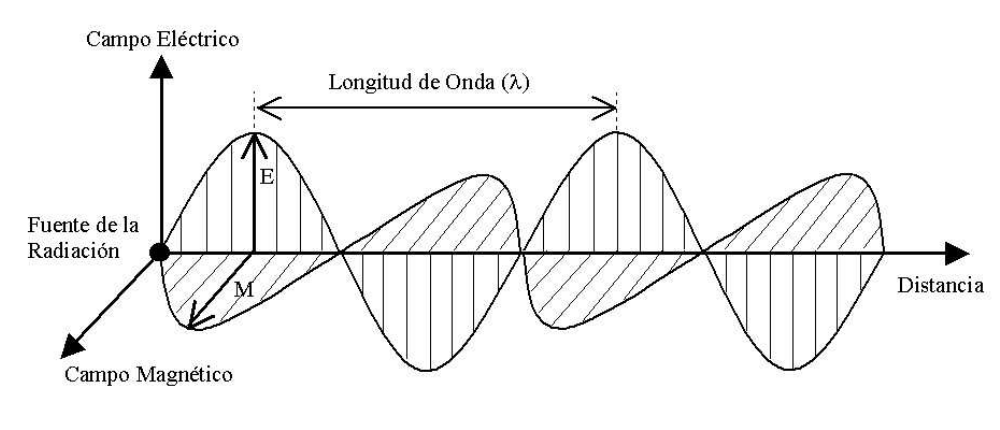
\includegraphics[width=.8\textwidth]{./images/propagacion.png}}
  \centering
  \caption{Se muestran los vectores eléctricos ($E$) y magnéticos ($M$), perpendiculares entre ellos,de una onda electromagnética. La longitud de onda ($\lambda$) corresponde a la distancia entre dos crestas consecutivas. \cite{chile}}
  \label{fPropagacion}
\end{figure}

Cuando se logra ver algo, no es directamente el objeto que se ve, sino la radiación electromagnética dentro del rango visual que emite dicho objeto y parte de la energía es absorbida por el objeto, ya que actúan con base en los componentes químicos que lo forman. El espectro electromagnético se divide en rangos(vea tabla \ref{tEspectro}).

También se le dice espectro electromagnético a la radiación electromagnética que absorbe o emite una sustancia. Dicha radiación sirve para identificar la sustancia de manera análoga a una huella dactilar lo cual será explicado en el siguiente subtema \ref{FirmasEspectrales}. Los espectros se pueden observar mediante espectroscopios que, además de permitir ver el espectro, permiten realizar medidas sobre el mismo, como son la longitud de onda, la frecuencia y la intensidad de la radiación.\\
Una cámara digital \textit{RGB} tradicional capta el espectro visible que responde a longitudes de onda 390 nm a 750 nm(vea la tabla \ref{tEV}). El objetivo de las cámaras tradicionales es dar como resultado una imagen en el rango de visibilidad humana. Lo interesante es cuando se toma en cuenta otros valores fuera del rango visible. (véase la Figura \ref{fNasa})

\begin{table}[]
\centering
\begin{tabular}{l|l|l|l|}
\cline{2-4}
                         & Color    & \begin{tabular}[c]{@{}l@{}}Intervalo de longitud\\ de onda ($\lambda$)\end{tabular} & \begin{tabular}[c]{@{}l@{}}Intervalo de \\ frecuencia ($\nu$)\end{tabular} \\ \cline{2-4}
\cellcolor[HTML]{FE0000} & Rojo     & $\sim$ 700 - 635 nm                                                               & $\sim$ 430 - 480 THz                                                 \\ \cline{2-4}
\cellcolor[HTML]{FFA500} & Naranja  & $\sim$ 635 – 590 nm                                                                & $\sim$ 480 – 510 THz                                                 \\ \cline{2-4}
\cellcolor[HTML]{FFFF00} & Amarillo & $\sim$ 590 – 560 nm                                                                & $\sim$ 510 – 540 THz                                                 \\ \cline{2-4}
\cellcolor[HTML]{008000} & Verde    & $\sim$ 560 – 520 nm                                                                & $\sim$ 540 – 580 THz                                                 \\ \cline{2-4}
\cellcolor[HTML]{00FFFF} & Cian     & $\sim$ 520 – 490 nm                                                                & $\sim$ 580 – 610 THz                                                 \\ \cline{2-4}
\cellcolor[HTML]{0000FF} & Azul     & $\sim$ 490 – 450 nm                                                                & $\sim$ 610 – 670 THz                                                 \\ \cline{2-4}
\cellcolor[HTML]{EE82EE} & Violeta  & $\sim$ 450 – 400 nm                                                                & $\sim$ 670 – 750 THz                                                 \\ \cline{2-4}
\end{tabular}
\caption{Espectro visible\cite{Craig}.}
\label{tEV}
\end{table}

\begin{table}[]
\centering
\begin{tabular}{|l|l|l|}
\hline
\multicolumn{1}{|c|}{\textbf{\begin{tabular}[c]{@{}c@{}}Región o Banda\\ Espectral\end{tabular}}} & \multicolumn{1}{c|}{\textbf{\begin{tabular}[c]{@{}c@{}}Longitud \\ de onda $\lambda$\end{tabular}}}         & \textbf{Características}                                                                                                                                                                                           \\ \hline
Rayos Gamma                                                                                       & \textless 0.03 nm                                                                                        & \multirow{2}{*}{\textit{\begin{tabular}[c]{@{}l@{}}Radiación completamente absorbida\\ por las capas superiores de la \\ atmósfera. No se utilizan en \\ teledetección.\end{tabular}}}                                                                                  \\ \cline{1-2}
\\Rayos X  \\                                                                                         & 0.03 - 30 nm                                                                                             &                                                                                                                                                                                                                                                                          \\ \hline
Ultravioleta (UV)                                                                                 & 0.03 - 0.4 $\mu$m                                                                                            & \textit{\begin{tabular}[c]{@{}l@{}}La radiación con $\lambda$ \textless 0.3 $\mu$m es\\ completamente absorbida por la capa\\ de ozono de la atmósfera.\end{tabular}}                                                                                                           \\ \hline
\begin{tabular}[c]{@{}l@{}}Visible (azul,verde\\ y rojo)\end{tabular}                             & \begin{tabular}[c]{@{}l@{}}0.4 - 0.5 $\mu$m (azul)\\ 0.5 - 0.6 $\mu$m (verde)\\ 0.6 - 0.7 $\mu$m (rojo)\end{tabular} & \textit{\begin{tabular}[c]{@{}l@{}}Se puede detectar a través de \\ fotodetectores y películas fotosensibles\\ normales (color B/N).\end{tabular}}                                                                                                                       \\ \hline
Infrarrojo reflejado                                                                              & \begin{tabular}[c]{@{}l@{}}0.7 - 1.3 $\mu$m \\ (IR cercano)\\ 1.3 - 3.0 $\mu$m \\ (IR medio)\end{tabular}        & \textit{\begin{tabular}[c]{@{}l@{}}Radiación solar reflejada que no\\ contiene información acerca de las\\ propiedades térmicas de los materiales.\\ El rango 0.7 a 0.9 $\mu$m se puede \\ detectar usando películas fotosensibles\\ (infrarrojo fotográfico).\end{tabular}} \\ \hline
Infrarrojo térmico                                                                                & \begin{tabular}[c]{@{}l@{}}3.0 - 5.0 um\\ 8.0 - 14.0 um\end{tabular}                                     & \textit{\begin{tabular}[c]{@{}l@{}}Corresponden a dos ventanas\\ atmosféricas en la región térmica.\end{tabular}}                                                                                                                                                        \\ \hline
\begin{tabular}[c]{@{}l@{}}Radar (región de \\ las microondas)\end{tabular}                       & 0.1 - 100 cm                                                                                             & \textit{\begin{tabular}[c]{@{}l@{}}Radiación de grandes longitudes de\\ onda, capaces de penetrar nubes,\\ nieblas y lluvia.\end{tabular}}                                                                                                                               \\ \hline
Ondas de Radio y TV                                                                               & \textgreater 100 cm                                                                                      & \textit{\begin{tabular}[c]{@{}l@{}}Radiación con las mayores longitudes\\ de onda del espectro. Se utilizan en \\ telecomunicaciones.\end{tabular}}                                                                                                                      \\ \hline
\end{tabular}
\caption{Descripción de las regiones del espectro electromagnético ($1 \mu m = 10^{-6}$ m y 1 nm = $10^{-9} m$)\cite{chile}.}
\label{tEspectro}
\end{table}


%Craig F. Bohren (2006). Fundamentals of Atmospheric Radiation: An Introduction with 400 Problems. Wiley-VCH. ISBN 3-527-40503-8.

\begin{figure}[h]
  \centering
  \framebox[14cm]{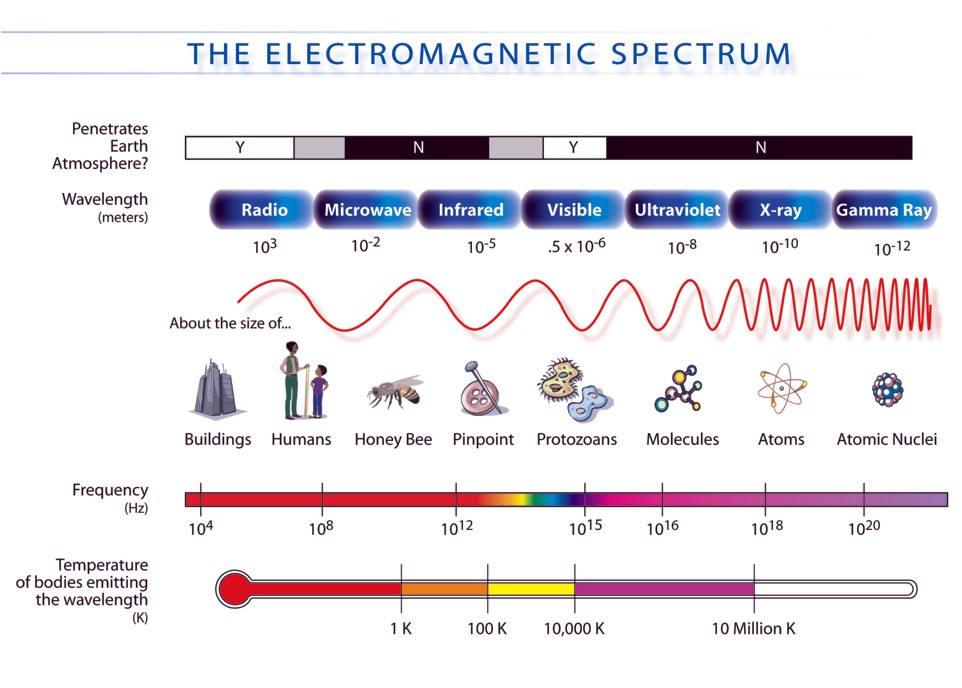
\includegraphics[width=.8\textwidth]{./images/nasa.jpg}}
  \centering
  \caption{Diagrama del espectro electromagnético \cite{nasaimage}.}
  \label{fNasa}
\end{figure}
\subsection{Firmas espectrales}
\label{FirmasEspectrales}
La firma espectral es la variación de reflectancia de la radiación proveniente de la energía solar cuando tiene contacto con la superficie terrestre reflejada, absorbida y transmitida. La energía es reflejada cuando es rebotada, es absorbida cuando conserva energía provocando calor en el material y es transmitida cuando pasa a través del material. Como se comentó en el capítulo anterior, el espectro electromagnético es dado por la radiación emitida y absorvida por el objeto. Gracias a que cada elemento capturado emite radiación electromagnética recibida del sol de forma diferenciada, es posible mediante un análisis de los datos determinar qué elementos químicos lo forman y determinar qué es lo que se capto, tal como se puede ver en la Figura \ref{fFirma}. \cite{AVIRIS}

\begin{figure}[h]
  \centering
  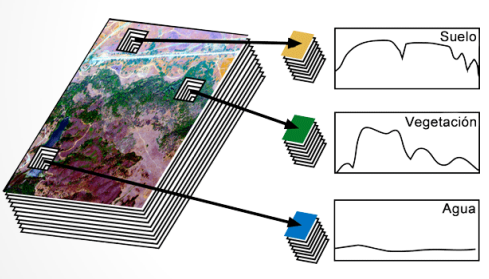
\includegraphics[width=.7\textwidth]{./images/firma.png}
  \centering
  \caption{Firmas espectrales de suelo, vegetación y agua. \cite{Quinones}.}
  \label{fFirma}
\end{figure}
%IMÁGENES HIPERESPECTRALES: ANÁLISIS Y APLICACIONES. Sebastián Quiñones F. Cartógrafo Centro de Ecología Aplicada
Otra de las aplicaciones muy comunes es detectar la sanidad de las plantas tomando en cuenta las variables ya mencionadas como se puede observar en un ejemplo en la Figura \ref{fSanidad}. También se han utilizado estas técnicas en detección de sanidad en animales \cite{animal} como se ve en la Figura \ref{fAnimal}. \cite{medical}

\begin{figure}[h]
  \centering
  \framebox[14cm]{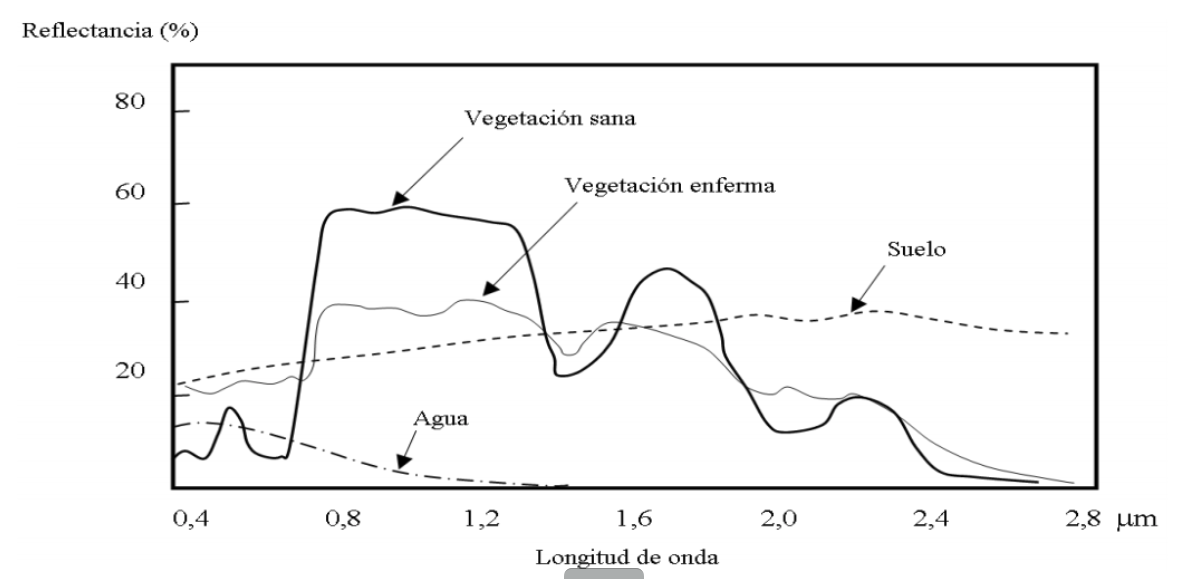
\includegraphics[width=.8\textwidth]{./images/sanidad.png}}
  \centering
  \caption{Detección de sanidad en vegetales \cite{chile}.}
  \label{fSanidad}
\end{figure}

\begin{figure}[h]
  \centering
  \framebox[5cm]{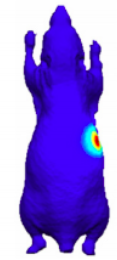
\includegraphics[width=.2\textwidth]{./images/animal.png}}
  \centering
  \caption{Detección espectral de anormalidades en animales. \cite{animal}.}
  \label{fAnimal}
\end{figure}
%Abhijit J Chaudhari and Felix Darvas and James R Bading and Rex A Moats and Peter S Conti and Desmond J Smith and Simon R Cherry and Richard M Leahy, “Hyperspectral and multispectral bioluminescence optical tomography for small animal imaging,” in Physics in Medicine and Biology, vol. 50, 2005
\subsection{Imagen espectral}
Tomando en cuenta que una imagen es la reproducción de una figura por la combinación de los rayos de luz y que el espectro es la radiación electromagnética que es absorbida o emitida, se puede concluir que una imagen espectral es la reproducción de una figura de un objeto por la combinación de radiación emitida en cierta longitud de onda electromagnética (véase la Figura \ref{fWiki}).

\begin{figure}[h]
  \centering
  \framebox[14cm]{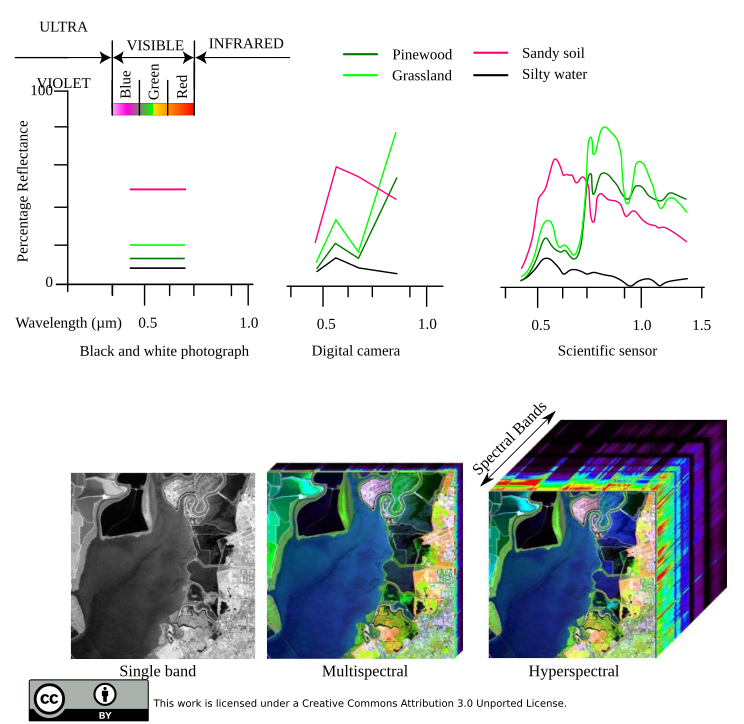
\includegraphics[width=.8\textwidth]{./images/wiki.png}}
  \centering
  \caption{Imagen hiperespectral, multiespectral y espectral.}
  \label{fWiki}
\end{figure}

\subsection{Imagen Multiespectral}
Las imágenes Multiespectrales son un conjunto de entre 3 a 20 imágenes de las mismas dimensiones (véase Figura \ref{fWiki}), reproduciendo una figura con base en diferentes rangos de longitud de onda electromagnética (véase la Figura \ref{fJairo}). Donde no necesariamente tienen que ser contiguas en los rangos tomados. Esto produce un arreglo de imágenes correspondientes a un mismo objeto o toma pero en diferentes longitudes de onda.

\begin{figure}[h]
  \centering
  \framebox[14cm]{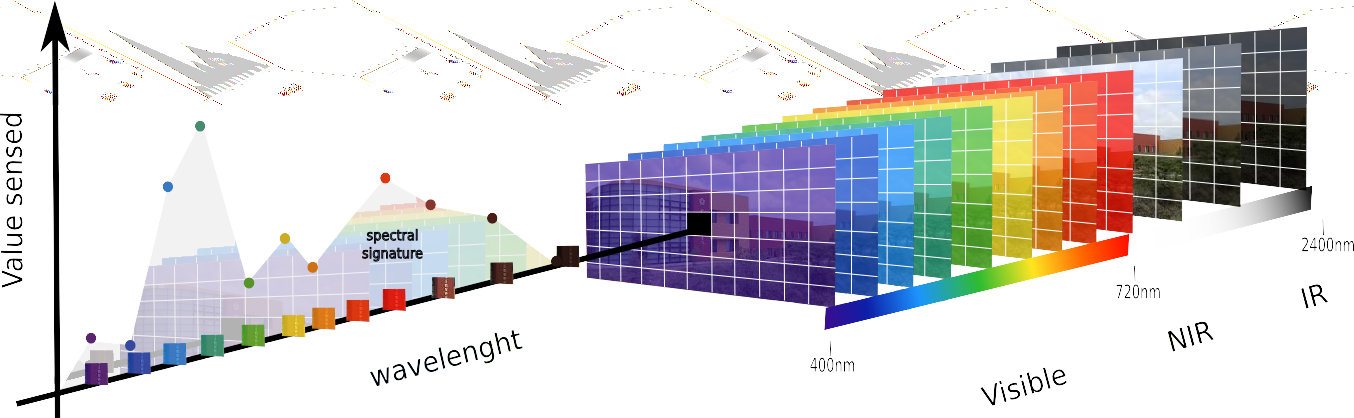
\includegraphics[width=.8\textwidth]{./images/jairo.png}}
  \centering
  \caption{Longitudes de onda \cite{FuzzyVD}.}
  \label{fJairo}
\end{figure}

\subsection{Imagen Hiperespectral}
El concepto de hiperespectral deriva de la toma de una gran cantidad de espectros de una superficie. Donde cada toma es obtenida para formar un cubo de la imagen.(véase la Figura \ref{fWiki})

Tomando en cuenta la información recolectada a lo largo del espectro electromagnético se forma un cubo de datos con el que se puede trabajar ya según la aplicación que se le quiera dar. Usando los principios de CTIS, la forma en que se captura una imagen hiperespectral es obteniendo el contenido espectral de cada pixel en una imagen 2D superposicionada. Esta tecnología divide los datos de la imagen pixel por pixel en bandas estrechas de longitud de onda, dando como resultado un cubo 3D de datos como se muestra en la Figura \ref{fPaper1}.\\

\begin{figure}[h]
  \centering
  \framebox[9cm]{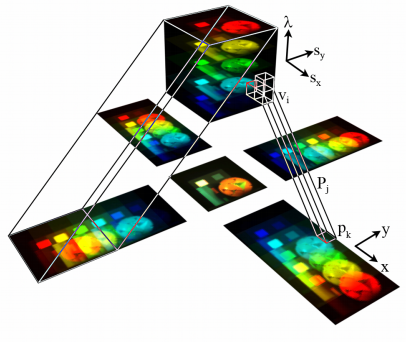
\includegraphics[width=.6\textwidth]{./images/paper1.png}}
  \centering
  \caption{Proyecciones paralelas de difracción \cite{PracCam}.}
  \label{fPaper1}
\end{figure}

\section{CTIS}
\label{CTIS}
El espectrómetro de imágenes por tomografía computarizada es utilizado para la captura de las imágenes hiperespectrales sin necesidad de escaneo puesto que es obtenido en un \textit{snapshot} que consiste en un único tiempo de integración gracias a un conjunto de detectores.
Funciona como si se tratara de dos cámaras en sí, donde una toma la imagen base en un cuadro de visión y la segunda capta la energía a distintas longitudes de onda electromagnética reflectada en el marco tomado.
Dando como resultado una imagen de referencia(zero mode) y los espectros captados a diferentes longitudes de onda basadas en dicha imagen.

Da como resultado una imagen 2D que es una superposición de los espectros, siendo el cubo hiperespectral proyectado de forma paralela en distintos ángulos (vea la Figura \ref{fPaper1}). El cubo formado es compuesto por voxeles ($V_i$), que son una unidad cúbica componente de la imagen hiperespectral definidos por la resolución de la imagen superposicionada.

La estructura del dispositivo CTIS son las presentadas en la Figura \ref{fCTIS}, donde la lente de imagen (\textit{imaging lens}) refleja la imagen a través de la apertura ya sea una imagen o conjunto de imágenes (\textit{slit/square aperture}). La luz divergente es hecha paralela al pasar por la \textit{lente de colimación} (\textit{collimation lens}), para después pasar por la rejilla de difracción (\textit{diffraction grating}). La luz difractada y no difractada se vuelven a hacer imágenes mediante el lente de reimagen (\textit{re-imaging lens}). Finalmente el resultante es captado por el sensor.

\begin{figure}[h]
  \centering
  \framebox[13cm]{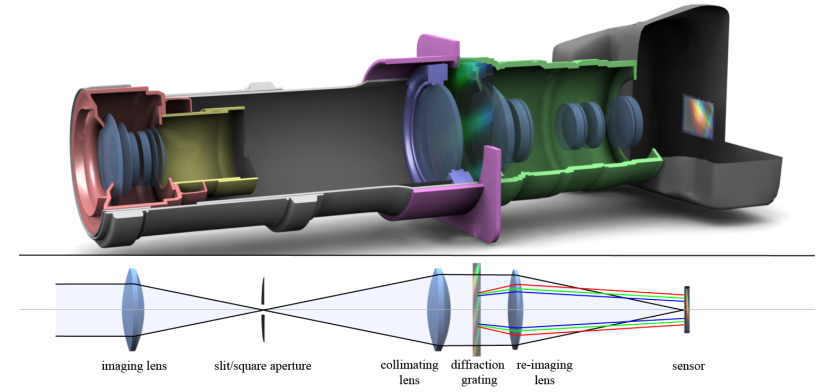
\includegraphics[width=.9\textwidth]{./images/CTIS.png}}
  \centering
  \caption{Estructura CTIS. \cite{PracCam}}
  \label{fCTIS}
\end{figure}

%Chapter 3 overview explain RGGB
\subsection{Calibración espacial}
%The spatial calibration localizes the positions of individual wavelenghts on the image grid (in slit mode), or determinesthe coefficients of the projection of the data cube.
%The calibration will allow a precise mapping from the projected image to wavelenghts in the spectrum.

La calibración espacial corrige distorsiones que tenga la imagen obtenida por el dispositivo CTIS. Lo que hace es buscar desalineamientos cuando pasa la luz entre la apertura y la rejilla de difracción.

\subsection{Calibración espectral}
%Calculates the spectral intensity response od the optical system and the sensor pixels. The pixels are arranged in a RGGB Bayer filter array, so each pixel responds more in the red, green or blue range of the spectrum. This means that similar to standard imaging, we need to apply demosaicing algorithms to recover the full spectra

El objetivo de la calibración espectral es ajustar la sensibilidad espectral de cada canal de color que se determinan identificando un espectro cuando es continuo y conocido con alta precisión.

\subsection{Medición de slit espectral e interpolación cromática}
Para la reconstrucción del verdadero espectro de la medición aplicando la calibración espectral $f(x,y)$ debemos tomar en cuenta las diferentes sensibilidades de los diferentes canales de color en el \textit{filtro Bayer} (\textit{Bayer filter} \cite{Bayer}).
Cualquier canal puede ser utilizado para reconstruir un espectro considerando que se tiene una respuesta por cada canal de color.
Puesto que la respuesta espectral de cada canal cubre sólo parte del espectro visible y las posiciones de los píxeles de Bayer están entrelazadas, se combinan las mediciones de píxeles de Bayer adyacentes con valores interpolados.
Para suprimir ruido los canales con peso (\textit{weight}) $W_{r,g,b}(\lambda)$ donde $r,g,b$ corresponden a los colores rojo(\textit{red}), verde(\textit{green}) y azul(\textit{blue}) basados en la amplitud de su respuesta espectral:
\begin{flalign}
  \label{FormulaMSS1}
  W_{r,g,b}(\lambda)=\frac{S_{r,g,b}(\lambda)}{\sum\limits_{c=r,g,b}S_{c}(\lambda)}.
\end{flalign}
después el espectro $M(\lambda)$ de una medida de respuesta $m_{r,g,b}(\lambda)$ es reconstruida con:
\begin{flalign}
  \label{FormulaMSS2}
  M(\lambda)=\sum\limits_{c=r,g,b}\frac{m_{c}(\lambda)}{S_{c}(\lambda)}w_{c}(\lambda)=\frac{\sum\limits_{c=r,g,b}m_{c}(\lambda)}{\sum\limits_{c=r,g,b}S_{c}(\lambda)}w_{c}(\lambda).
\end{flalign}
con valores interpolados donde fueron necesarios.


\subsection{Calibración hiperespectral}
La calibración hiperespectral consiste en usar la apertura cuadrada, puesto que tomando la apertura \textit{slit} solo se podrá tener una imagen a una cierta longitud de onda. En cambio utilizando la apertura cuadrada se podrá tomar un conjunto de imágenes a lo largo del espectro electromagnético, logrando así el cubo de datos.
\subsubsection{Teoría de reconstrucción CTIS} \cite{extra6} \cite{extra7}
Para la reconstrucción se toma en cuenta una matriz $H$ generada por la proyección paralela (vea capítulo \ref{CTIS}) que trabaja con el vector $\vec{f}$ que contiene voxeles del cubo de datos como se mostró en la Figura \ref{fPaper1}. $H$ es una matriz $M$ x $N$ donde $M$ es el número de píxeles en la imagen y $N$ el número de voxeles en el cubo de datos. Multiplicando la matriz por el vector $\vec{f}$ se obtiene un nuevo vector $\vec{g}$:
\begin{flalign}
  \label{FormulaCH1}
  \vec{g}=H\vec{f}.
\end{flalign}
Cada columna contiene cinco entradas en las posiciones difractadas que son la superior, inferior, a la izquierda, a la derecha y en el centro (zero mode). Como resultante de lo mencionado la matriz $H$ es muy grande por lo que se invierte la ecuación \ref{FormulaCH1}. Con la matriz $H$ se genera una primera suposición a través de $\vec{\hat{f}}0=H^T\vec g$ y se realiza la etapa iterativa de maximización de expectativas:
\begin{flalign}
  \label{FormulaCH2}
  \hat{f}_{n}^{k+1}=\frac
            {
              \hat{f}_{n}^{k}
            }
            {
              \sum\limits_{m=1}^{M}H_{mn}
            }
            \sum\limits_{m=1}^{M}
              H_{nm}^{T}
            \frac
            {
              g_{m}
            }
            {
              (H\hat{f}^{k})_{m}
            }.
\end{flalign}

\subsubsection{Calibración espacial hiperespectral}
Para calibrar la imagen hiperespectral se deberán tener identificadas las proyecciones correspondientes a cada espectro en las cinco entradas. Con base en la Figura \ref{fPaper1} se identifica la correspondencia de las proyecciones con base en las coordenadas $(x,y)$ de la imagen plana.
Si se deja a $P_{j}$ como proyecciones del cubo de datos $P_{j}(s_{x},s_{y},\lambda) = (x,y)$ construido por los voxeles $v_{i}=(s_{x_{i}},s_{y_{i}},\lambda_{i})$ que da cinco píxeles $p_k=(x_k,y_k)$ con índices $k \in 1...M$. Entonces $H$ puede ser construido mediante las cinco entradas $p_{k_1},...,p_{k_5}$ en la i-ésima columna de $H$ a uno.

Para que esto suceda se necesita determinar la posición de las cinco proyecciones para identificar alguna inclinación que tenga la imagen y poderlo revertir. Se toma una captura siendo $P_{0}$ el modo zero y $P_{1..4}(s_x,s_y,\lambda) = (x,y)$ (vea Figura \ref{fPaper1}), se alinean las $P_{1..4}$ en forma de cruz tomando como referencia central a $P_{0}$ mediante una interpolación lineal.

\subsubsection{Medición de imágenes hiperespectrales}
Al tener una imagen hiperespectral CTIS se necesita hacer una medición de las señales a distintas longitudes de onda para de esta forma identificar las caractarísticas superposicionadas de las diversas longitudes de ondas del espectro electromagnético.

Teniendo la matriz $H$ definida se puede proseguir para la solución de una imagen CTIS. Considerando que la utilización de la ecuación \ref{FormulaCH2} da una gran cantidad de ceros se tienen datos y procedimientos innecesarios. Para solucionar esto se propone separar por canal el arreglo de \textit{Mosaico de Bayer} tratando a los dos canales de verde (\textit{green} G) del \textit{arreglo Bayer RGGB}. Se realiza lo mismo con la matriz $H$ para extraer $H$ matrices para cada uno de los cuatro canales \textit{RGGB} solo para las longitudes de onda donde la correspondencia no sea cero.

\subsubsection{Interpolación cromática espacial y reconstrucción}
\label{Reconstruction}
La \textit{interpolación cromática} (\textit{demosaicing}) es el proceso que se realiza a un conjunto de muestras cromáticas tomadas de un sensor de imagen para producir una imagen a color.
Una vez realizada la interpolación cromática se podrá hacer la reconstrucción en la imagen CTIS.
Para lograr la reconstrucción se realiza una interpolación cromática, similar a la \textit{interpolación cromática} con imágenes RGB.
Posterior a ello se hace una interpolación bilineal para obtener los píxeles Bayer.
Una interpolación cromática espectral es diferente a las convencionales, por su información en superposición contenida.
Con el cubo de datos interpolados cromáticamente se recuperan los píxeles espectrales utilizando la ecuación \ref{FormulaMSS1}.
Mediante la configuración \textit{slit} se recolectan los valores por espectro, provocando de esta forma una integral para calcular la información en $S_{r,g,b}^l(\lambda_i)$ en resoluciones bajas:
\begin{flalign}
  \label{FormulaSDR}
  S_{r,g,b}^l(\lambda_i)=\int _{\lambda_i-\frac{r}{2}}^{\lambda_i+\frac{r}{2}}S_{r,g,b}(\lambda)d\lambda.
\end{flalign}

\cite{extra2}


\section{Mosaico de Bayer\cite{Bayer}}
El mosaico de Bayer es la interpolación en la imagen de dos muestras verdes, una roja y otra azul. Se tomó en cuenta el patrón Bayer \textit{RGGB} dejando en porcentaje 50\% de filtros verdes, un 25\% de rojos y un 25\% de azules en la imagen. La razón por la que se utilizan más muestras verdes es porque el ojo humano es más sensible a ese color.

Siendo el verde que aparece en todas las filas, los colores azul y rojo aparecen por fila uno y después el otro, denominando la fila roja cuando tiene rojo y verde, y fila azul cuando tiene azul y verde. Los verdes pueden aparecen en la posición par o la impar, alterado por el color de fila que se encuentre.
La fila con rojo tendría el patrón rojo, verde,rojo,verde,..., y el la fila con azul el patrón verde, azul, verde, azul,...

El patrón está desplegado en la Figura \ref{fBayer}.

\begin{figure}[h]
  \centering
  \framebox[9cm]{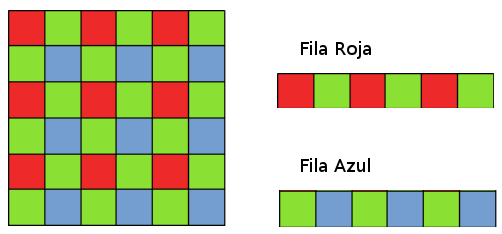
\includegraphics[width=.6\textwidth]{./images/Bayer.png}}
  \centering
  \caption{Patrón de Bayer.}
  \label{fBayer}
\end{figure}
%\subsection{Pseudocódigo}

%aplicado a imágenes wavelets0.
\section{Método de Malvar, He y Cutler}\label{capMalvar}
El método propuesto por Malvar, He y Culter deriva de una modificación de la interpolación bilineal e intenta atacar los problemas de la interpolación cromática. El algoritmo propuesto consta de un simple método lineal usando filtros 5x5. Para la interpolación cromática se utilizará la imagen pasada por una matriz de filtros de color (en inglés \textit{Color Filter Array} CFA) Bayer pattern\cite{Bayer}.

En localización del azul o rojo pixel, la interpolación bilineal del componente verde es el promedio de sus cuatro vecinos axiales,
\begin{flalign}
  \label{Malvar1}
  \hat{G}^{bl}(i,j)=
  \frac{1}{4}(
  G(i-1,j)+
  G(i+1,j)+
  G(i,j-1)+
  G(i,j+1)
  ).
\end{flalign}
La interpolación bilineal de los componentes azul y rojo son similares, la diferencia es que toman a sus cuatro vecinos diagonales.

La localización del componente verde en el pixel rojo está estimado como
\begin{flalign}
  \label{Malvar2}
  \hat{G}(i,j)=\hat{G}^{bl}(i,j)+\alpha \Delta _R(i,j),
\end{flalign}
donde $\Delta _R$ es el \textit{Laplaciano} discreto de cinco puntos del canal rojo,
\begin{flalign}
  \label{Malvar3}
  \Delta _R(i,j):=R(i,j)-\frac{1}{4}(R(i-2,j)+R(i+2,j)+R(i,j-2)+R(i,j+2)).
\end{flalign}
Para estimar el componente rojo en la localización del pixel verde,
\begin{flalign}
  \label{Malvar4}
  \hat{R}(i,j)=\hat{R}^{bl}(i,j)+\beta \Delta _G(i,j),
\end{flalign}
donde $\Delta _G$ es el Laplaciano discreto de nueve puntos del canal verde.
Para estimar un componente rojo en una localización de un pixel azul,
\begin{flalign}
  \label{Malvar5}
  \hat{R}(i,j)=\hat{R}^{bl}(i,j)+\gamma \Delta _B(i,j),
\end{flalign}
donde $\Delta _B$ es el discreto Laplaciano de cinco puntos del canal azul.

Los parámetros de $\alpha$, $\beta$ y $\gamma$ controlan el peso de los términos de conección Laplacianos,
\begin{flalign}
  \label{Malvar6}
  \alpha =\frac{1}{2},\text{  }\beta =\frac{5}{8},\text{  }\gamma \frac{3}{4}.
\end{flalign}


\section{Gaussian blur\cite{Blur}}\label{CapBlur}
El desenfoque Gaussiano (Gaussian blur) es un método que utiliza algorítmos matemáticos. Se basa en la función Gaussiana,
\begin{flalign}
  \label{Gauss1}
  f(x)=ae-\frac{{(x-b)}^2}{2c^{2}}
\end{flalign}
que aplicado a las imágenes mezcla poco los colores de los vecinos de los píxeles entre sí. Lo cual ocasiona que se pierdan detalles y se vea incluso borroso.
Para la aplicación de esta función en las imágenes utilizadas en el proyecto se utilizó matlab.

\section{Sharpender\cite{Sharp}}\label{capSharpender}
La nitidez(sharpender) es el proceso inverso a desenfoque, puesto que intenta dar forma a bordes y a detalles de la imagen.
Pretende dar más calidad en la imagen resaltando pequeños contrastes en los píxeles con respecto a sus vecinos.
Para la aplicación de esta función en las imágenes utilizadas en el proyecto se utilizó matlab.
\section{GPA}
El algorítmo Análisis General Anterior(en inglés \textit{General Analysis Prior} GAP) para la reducción de ruido impulsivo para imágenes hiperespectrales está basado en la minimización de la variación total.\cite{MatlabDenoising}
\subsection{Transformada de Fourier}
Las transformadas de Fourier han jugado un papel importante al referirse a algoritmos de reconstrucción y filtrado de imágenes. A continuación se dará un repaso a las series de Fourier que después serán referenciadas en uno de los algoritmos de filtrado de imágenes utilizado en el presente proyecto.
\subsubsection{Series de Fourier \cite{FourierBook}}
Una función periódica $g(x)$ con un periodo $T$ tal que
\begin{flalign}
	\label{Fourier1}
	g(x)=g(x+T), -\infty  < x < \infty
\end{flalign}
podrá ser representada como una serie de Fourier:
\begin{flalign}
	\label{Fourier2}
	g(x)=\sum \limits_{n=-\infty}^{\infty}G_{n}e^{\frac{i2\pi nx}{T}}.
\end{flalign}
La función $g(x)$ deberá ser integrable en un periodo y ser continua. La función $g(x)$ deberá tener extremos en un periodo.
El coeficiente $G_{n}$ puede ser determinado por la siguiente relación ortogonal:
\begin{flalign}
	\label{Fourier3}
	\int_{-\frac{T}{2}}^
	{\frac{T}{2}}
	dx\text{ }
	e^{\frac{i2\pi (m-n)x)}{T}}
	=
	\left [
	\frac
	{e^{\frac{i2\pi (m-n)x)}{T}}}
	{\frac{i2\pi (m-n))}{T}}
	\right ]_
	{-\frac{T}{2}}^
	{\frac{T}{2}}=
	T \frac{\sin \pi (m-n))}{\pi (m-n))}=
	T\delta _{m,n}
\end{flalign}
Los coeficientes $G_n$ pueden ser obtenidos como:
\begin{flalign}
	\label{Fourier4}
	G_n=\frac{1}{T}\int _{-\frac{T}{2}}^{\frac{T}{2}}dx\text{ }g(x)e^{\frac{-i2\pi nx}{T}}.
\end{flalign}
Si $g(x)$ tiene una discontinuidad en $x=x_0$, la expanción de la serie converge a:
\begin{flalign}
	\label{Fourier5}
	g(x_0)=\frac{g(x_{0-})+g(x_{0+})}{2}.
\end{flalign}
Todos los términos impares son utilizados, por lo que la expansión de la serie de Fourier queda así:
\begin{flalign}
	\label{Fourier6}
	g(x)=\frac{1}{2}+\frac{2}{\pi}sin(\frac{2\pi x}{T})+\frac{2}{3\pi}sin(\frac{6\pi x}{T})+...
\end{flalign}
Las tramas producidas por la serie converge a una onda cuadrada. En la Figura \ref{fFourier} se puede ver como al agregar más términos de la serie se produce la convergencia.

\begin{figure}[h]
  \centering
  \framebox[9cm]{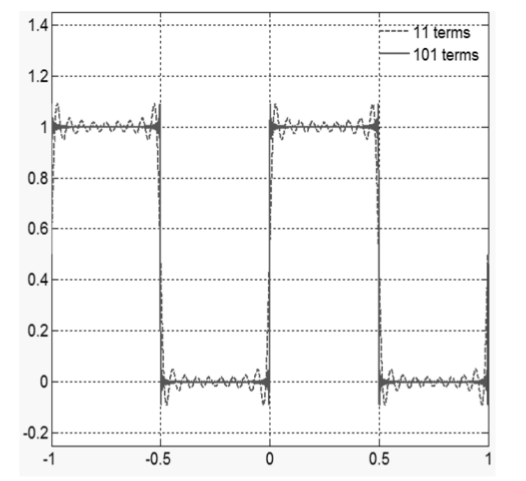
\includegraphics[width=.6\textwidth]{./images/fourier.png}}
  \centering
  \caption{Onda cuadrada representación de serie de Fourier con 11 y 101 terminos como en la ecuación \ref{Fourier6} \cite{FourierBook}.}
  \label{fFourier}
\end{figure}

%\subsubsection{Fenómeno de Gibbs}

\subsection{Transformadas de Wavalet} \cite{extra10}\cite{extra11}
Las wavelets son prácticamente mini ondas a diferencia de las infinitas como seno y coseno. La finalidad de que sean cortas es que puedan desvanecer rápidamente, limitadas en tiempo y frecuencia. A diferencia de la transformada de Fourier siendo infinita, la transformada de Wavalet es desarmada usando el mismo wavalet a diferentes escalas en vez de usar la misma frecuencia de seno vea Figura \ref{fWvsF}.

\begin{figure}[h]
  \centering
  \framebox[9cm]{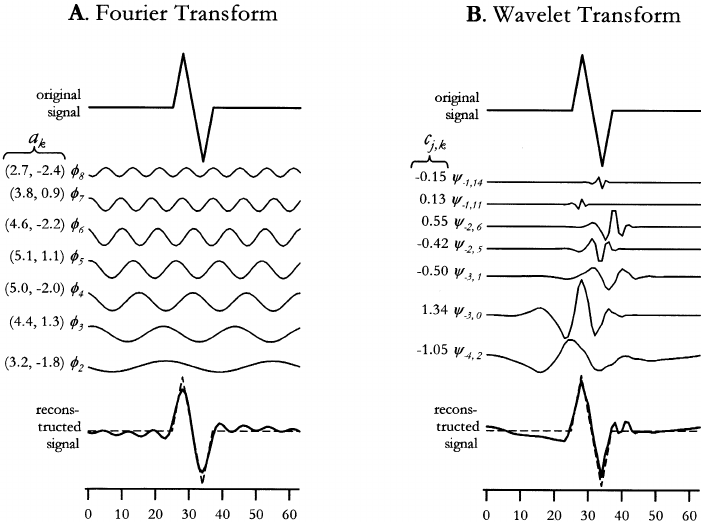
\includegraphics[width=.6\textwidth]{./images/waveletvsfft.png}}
  \centering
  \caption{Comparación entre transformada de Fourier y Wavelet \cite{WaveVsFourier}.}
  \label{fWvsF}
\end{figure}

Llamese $\varphi$ una base ortogonal del subespacio por escalación y transición se presenta la ecuación

\begin{flalign}
	\label{Dau1}
	\varphi _{i,j}(t)=\frac{1}{\sqrt{2}}\sum_{k\in \mathbf{Z}}h_k\varphi_{j+1,k}(t),
\end{flalign}

 siendo las funciones wavelets $\psi_{i,k}(t)$,  donde

 \begin{flalign}
	\label{Dau2}
	\psi_{i,k}(t)=\frac{1}{\sqrt{2}}\sum_{k\in \mathbf{Z}}g_k \varphi_{i+1,k}(t).
\end{flalign}

Se puede definir una transformada Wavelet como $f(t)$, donde

 \begin{flalign}
	\label{Dau3}
	f(t)=\sum_{j=0}^{J-1}\sum_{k=0}^{2^j-1}\omega _{j,k}\psi_{J,k}(t)+\sum_{k=0}^{L-1}s_{J,k}\varphi_{J,k}(t).
\end{flalign}

\subsubsection{Daubechies}\cite{Yakovlev} \label{rDau}%http://wwwmayr.in.tum.de/konferenzen/Jass05/courses/2/Yakovlev/Yakovlev_paper.pdf
Para obtener las transformadas Daubechies es necesario aplicar condiciones de momentos nulos(zero moments) a la función Wavelet que se le llamará función padre. Para hacer esto se deberán tener presentes las siguientes condiciones:

\begin{flalign}
  \label{Dau3}
  \left\{\begin{matrix}
  h_0+h_1+h_2+h_3=\sqrt{2}
  \\ h_1+2h_2+3h_3=0
  \\ h_0^2+h_1^2+h_2^2+h_3^2=1
  \\ h_0h_2+h_1h_3=0
\end{matrix}\right.
\end{flalign}
donde las soluciones serían:
\begin{flalign}
	\label{Dau3}
	h_0=\frac {1+\sqrt{3}}{4\sqrt{2}},\text{  }
	h_1=\frac{3+\sqrt{3}}{4\sqrt{2}},\text{  }
	h_2=\frac{3-\sqrt{3}}{4\sqrt{2}},\text{  }
	h_3=\frac{1-\sqrt{3}}{4\sqrt{2}}.
\end{flalign}

En la Figura \ref{fDau} se puede observar un ejemplo de \textit{wavelength} aplicando las condiciones de momentos nulos en contraste con una función general Wavelet.

\begin{figure}[h]
  \centering
  \framebox[9cm]{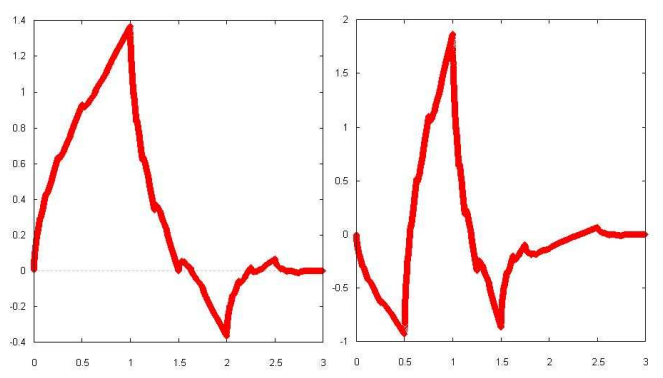
\includegraphics[width=.6\textwidth]{./images/dau.png}}
  \centering
  \caption{Daubachies y función wavelet \cite{Yakovlev}.}
  \label{fDau}
\end{figure}
%http://wwwmayr.in.tum.de/konferenzen/Jass05/courses/2/Yakovlev/Yakovlev_paper.pdf
%Marco Teórico
\chapter{Propuesta} % Main chapter title
\label{Capitulo3} % Change X to a consecutive number; for referencing this chapter elsewhere, use \ref{ChapterX}
\lhead{\emph{Propuesta}}

%----------------------------------------------------------------------------------------
%	SECTION 1
%----------------------------------------------------------------------------------------
%algorithm uses Daubechies wavelet for spatial dimension and Fourier transform for vertical dimension. 
\section{Proceso}
Como se pudo capitalizar en el marco teórico del documento, los diversos pasos para llegar al resultado esperado constan de mejoras que se realizarían después de la etapa de obtención de los las imagenes hiperespectrales realizadas por la camara con estructura CTIS. Los métodos (o por decir de otra forma, filtros) son independientes entre sí, por lo que uno de ellos no necesita de la ejecución de otro previo para poderse aplicar. 
La propuesta se basa en utilizar uno, o combinación de los siguientes métodos encontrando así el mejor camino hacia el resultado esperado:

\begin{itemize}
\item Daubichies.
\item Slices.
\item Mosaic-Malvar.
\item Blur-Shparpender.
\end{itemize}

Donde cada uno de dichas combinaciones será probada por la calidad percibida mediante el ojo humano. 
Para poder analizar las imágenes se establecieron rutas de resultados que se muestran en la Figura \ref{pics:squeme}, donde se utilizaron diversas combinaciones de la teoría mostrada en los capítulos anteriores.
\clearpage
\begin{figure}[h]
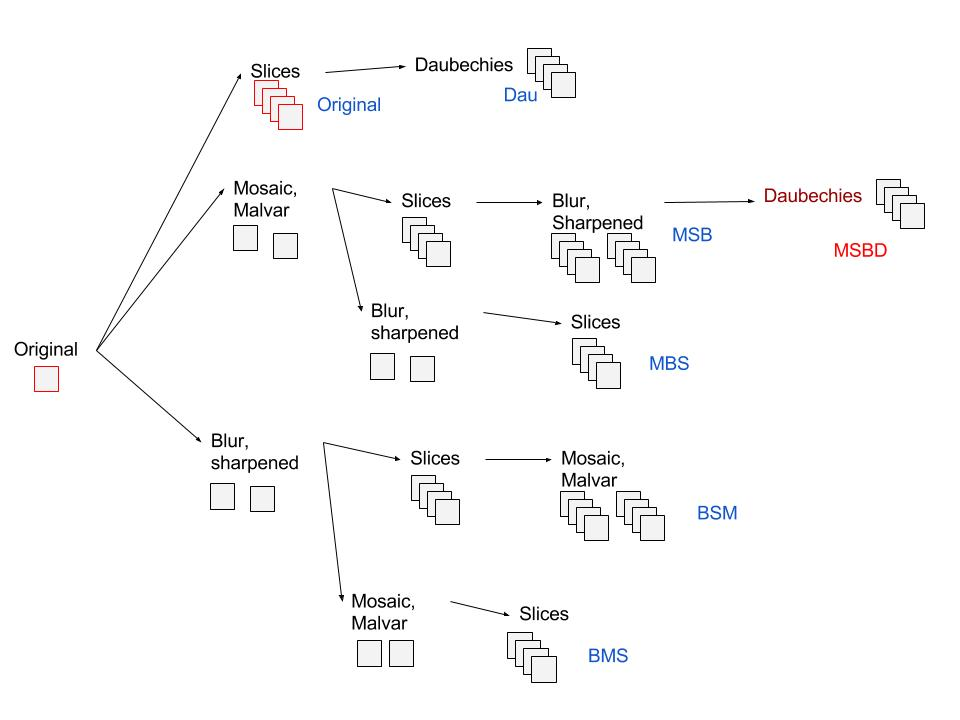
\includegraphics[scale=.4]{./images/RESULTS/squeme.jpg}
\caption{Esquema de resultados.}
\label{pics:squeme}
\end{figure}
Cada cuadro corresponde a una imagen superposicionadas y el conjunto de imágenes a las obtenidas por el procedimiento de abstracción por longitud de onda electromagnética de la imagen suporposicionada. %Algoritmo generador

\chapter{Resultados} % Main chapter title
\label{Capitulo4}
\lhead{\emph{Resultados}}

\section{Imágenes obtenidas}
La Figura \ref{pics:originalHDR} muestra la imagen HDR captada por la cámara hiperespectral de donde fueron sacadas las diversas imágenes por longitud de onda espectral mostradas en la Figura \ref{pics:slices}. La toma fue adquirida mediante la utilización de la cámara hiperespectral que fue utilizada mediante el uso de un software especializado, controlando dicho aparato. La toma fue una sola, que captó un marco de visión a diversas longitudes de onda.
\begin{figure}[h]
\begin{center}
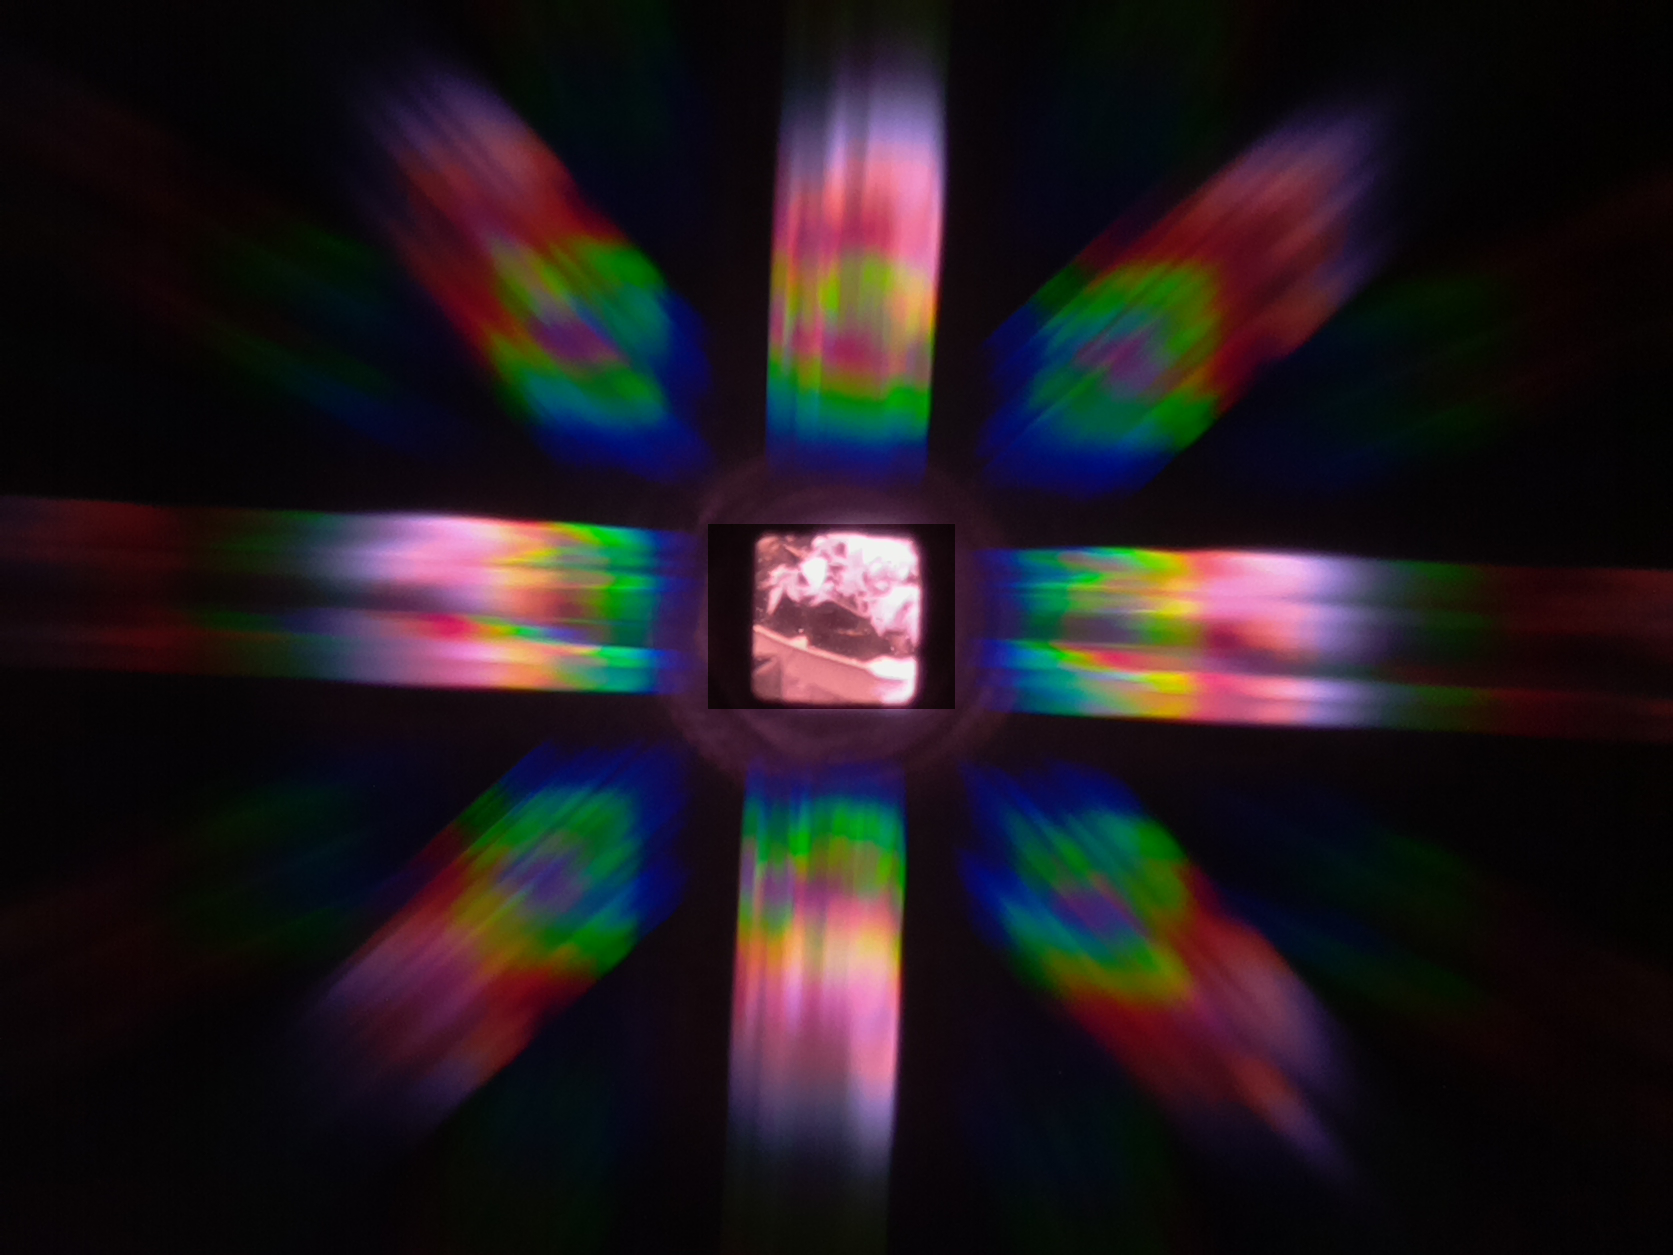
\includegraphics[scale=.3]{./images/RESULTS/original.png}
\end{center}
\caption{Imagen obtenida con camara hiperespectral.}
\label{pics:originalHDR}
\end{figure}

\begin{figure}[h]
\begin{center}$
\begin{array}{lll}
\subfloat[Imagen 466-637]{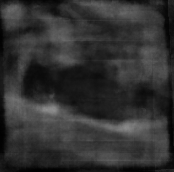
\includegraphics[scale=.99]{./images/RESULTS/slices/466.png}}&
\subfloat[Imagen 508-867]{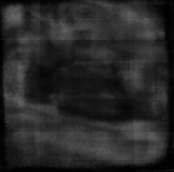
\includegraphics[scale=.99]{./images/RESULTS/slices/508.png}}&	
\subfloat[Imagen 549-087]{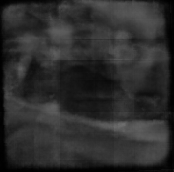
\includegraphics[scale=.99]{./images/RESULTS/slices/549.png}}
\end{array}$
\end{center}

\begin{center}$
\begin{array}{lll}
\subfloat[Imagen 589-307]{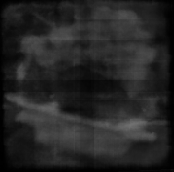
\includegraphics[scale=.99]{./images/RESULTS/slices/589.png}}&
\subfloat[Imagen 627-516]{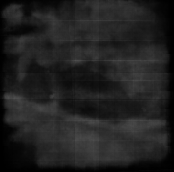
\includegraphics[scale=.99]{./images/RESULTS/slices/627.png}}&
\subfloat[Imagen 669-746]{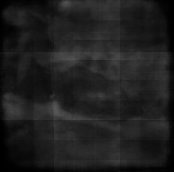
\includegraphics[scale=.99]{./images/RESULTS/slices/669.png}}
\end{array}$
\end{center}

\begin{center}$
\begin{array}{lll}
\subfloat[Imagen 709-966]{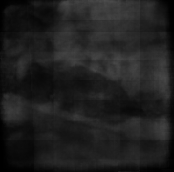
\includegraphics[scale=.99]{./images/RESULTS/slices/709.png}}&
\subfloat[Imagen 750-186]{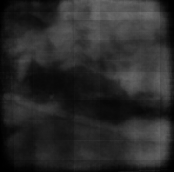
\includegraphics[scale=.99]{./images/RESULTS/slices/750.png}}&
\subfloat[Imagen 790-406]{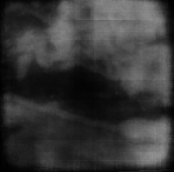
\includegraphics[scale=.99]{./images/RESULTS/slices/790.png}}
\end{array}$
\end{center}

\begin{center}$
\begin{array}{lll}
\subfloat[Imagen 830-625]{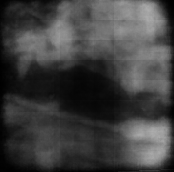
\includegraphics[scale=.99]{./images/RESULTS/slices/830.png}}&
\subfloat[Imagen 870-845]{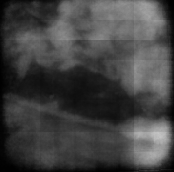
\includegraphics[scale=.99]{./images/RESULTS/slices/870.png}}&
\subfloat[Imagen 911-065]{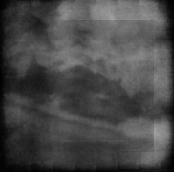
\includegraphics[scale=.99]{./images/RESULTS/slices/911.png}}
\end{array}$
\end{center}
\caption{Slices originales.}
\label{pics:slices}
\end{figure}

\clearpage
Con base en la Figura \ref{pics:squeme} los resultados tomados en consideración fueron el "Dau" que consta en aplicarle a los slices (conjunto de imágenes obtenidas mediante el método de obtención de imágenes por espectro CTIS) de la imagen hiperespectral el filtro utilizando la teoría de Daubichies (cápitulo \ref{rDau}), el MSB que consiste en la aplicación a la imagen original el Mosaic-Malvar y a ese resultado convertir la imagen HDR en slices para posterior aplicarle el Blur-Sharpened, además el MBS que de igual manera comienza aplicando el método de Moisac-Malvar seguido por el Blur-Sharpened y a ello después sacar los slices de la imagen hiperespectral, también el BSM que constaba en aplicarle a la imagen original el Blur-Sharpened seguido de sacar los slices y a ellos aplicarle el Mosaic-Malvar y por final se tomó el resultado BMS que era aplicarle a la imagen original el Bayer-Shapened y a ese resultado el Mosaic-Malvar para sacar los slices de la imagen superposicionada.

Para comparar los resultados se tomaron solo la imagen 870-845. Dichos resultados se muestran en la Figura \ref{pics:comparation}.

\begin{figure}[h]
\begin{center}$
\begin{array}{lll}
\subfloat[Original]{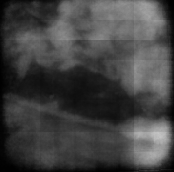
\includegraphics[scale=.99]{./images/RESULTS/compare870/original.png}}&
\subfloat[Dau]{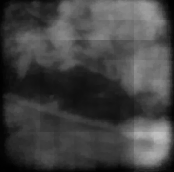
\includegraphics[scale=.7419]{./images/RESULTS/compare870/Dau.png}}&
\subfloat[MSB]{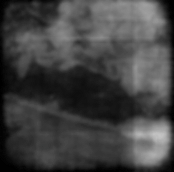
\includegraphics[scale=.7419]{./images/RESULTS/compare870/MSB.png}}
\end{array}$
\end{center}

\begin{center}$
\begin{array}{lll}
\subfloat[MBS]{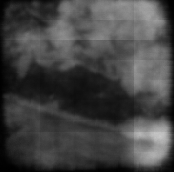
\includegraphics[scale=.99]{./images/RESULTS/compare870/MBS.png}}&
\subfloat[BSM]{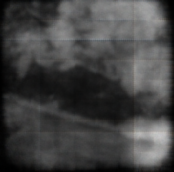
\includegraphics[scale=.7419]{./images/RESULTS/compare870/BSM.png}}&
\subfloat[BMS]{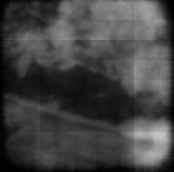
\includegraphics[scale=.99]{./images/RESULTS/compare870/BMS.png}}
\end{array}$
\end{center}

\caption{Comparación de resultados en imagen 870-845.}
\label{pics:comparation}
\end{figure}

Los resultados por los que se fueron obteniendo las imagenes se muestran en la Figura \ref{pics:process}, donde la imagen M es la imagen HDR original sometida a Malvar, MS es el resultado anterior sometido a el procedimiento de extracción de cubos. De ahí los slices se somente a Blur y sharpened resultando la imagen a comparar MSB. Y para finalizar el procedimiento se somete a la transformadas Daubichies para un último filtro dando como resultado la imagen MSBD.

\begin{figure}[h]
\begin{center}
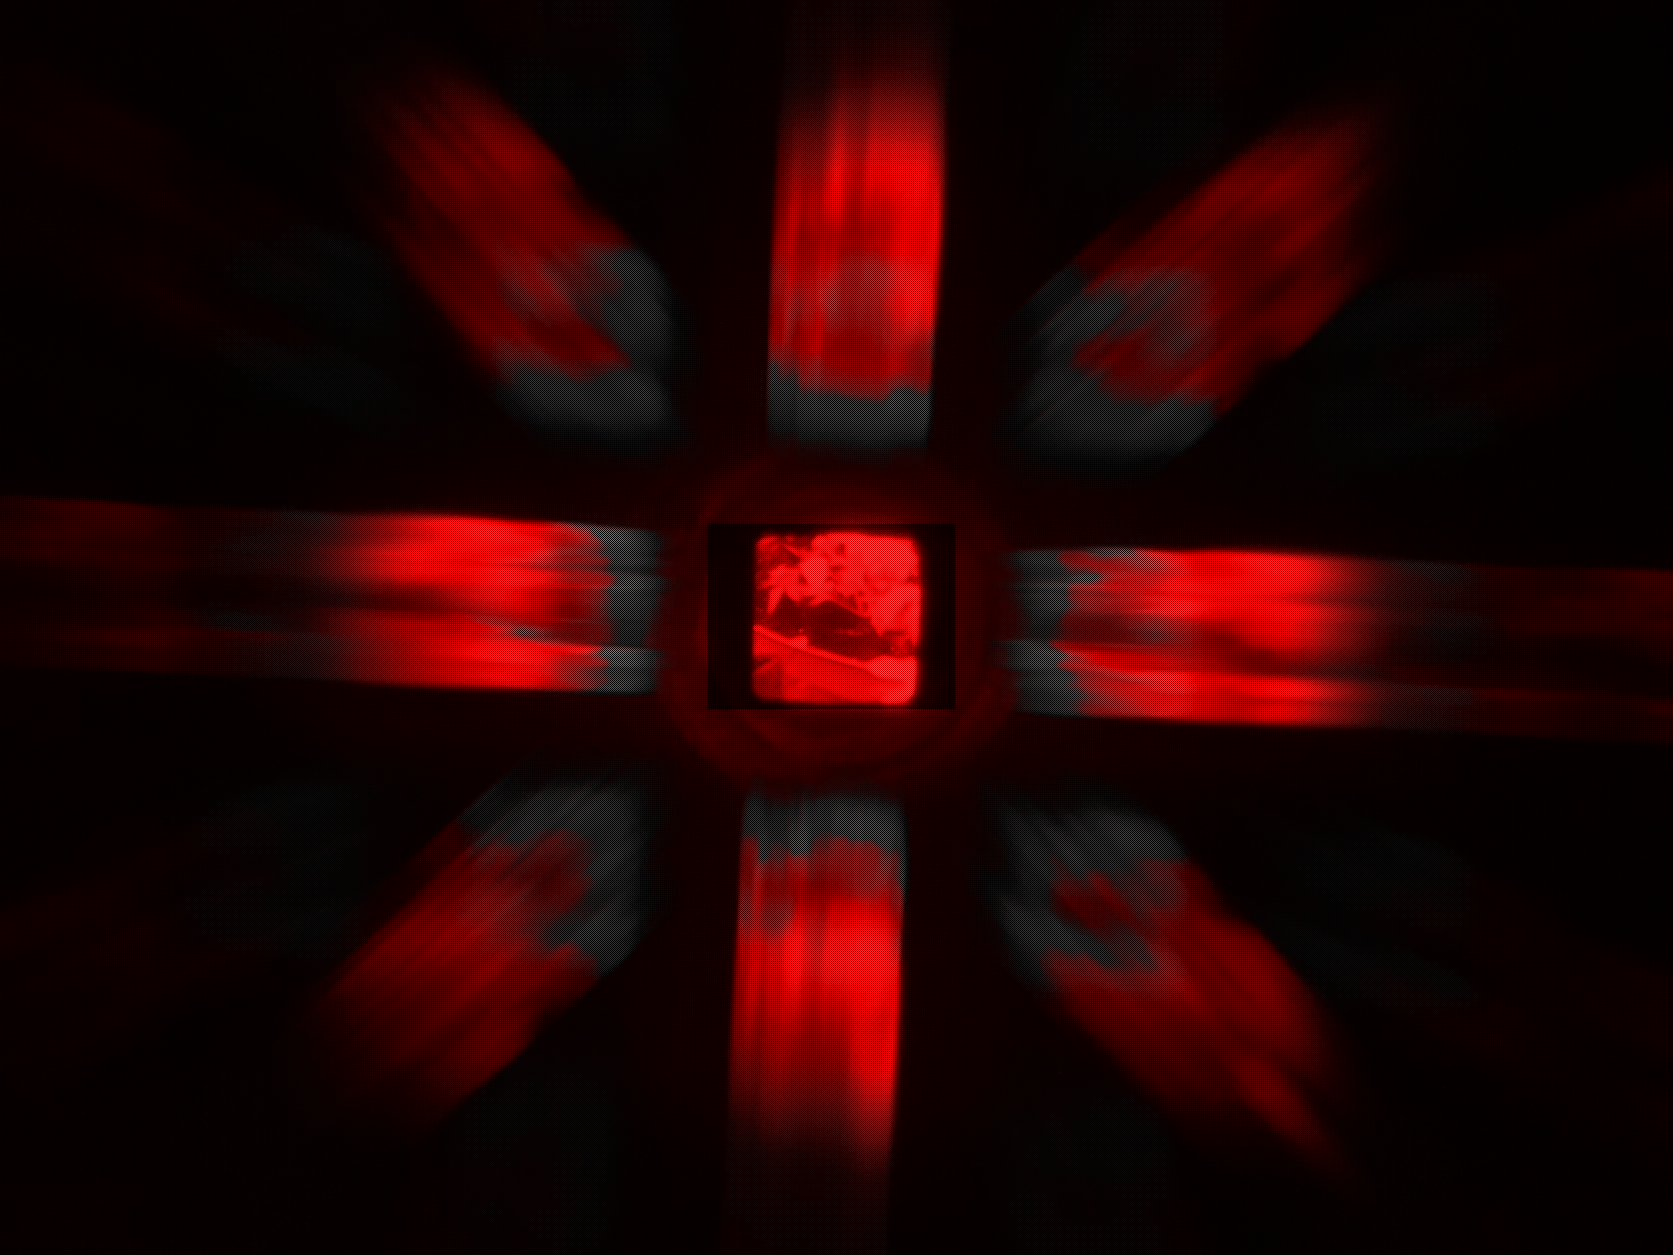
\includegraphics[scale=.2256]{./images/RESULTS/Malvar/mosaic.png}
\end{center}
\caption{Imagen obtenida con camara hiperespectral.}
\label{pics:originalHDR}
\end{figure}

\clearpage
\begin{figure}[h]
\begin{center}$
\begin{array}{lll}
\subfloat[MS]{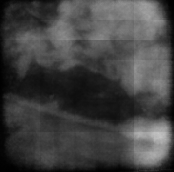
\includegraphics[scale=1.5]{./images/RESULTS/compare870/MS.png}}
\end{array}$
\end{center}

\begin{center}$
\begin{array}{lll}
\subfloat[MSB ]{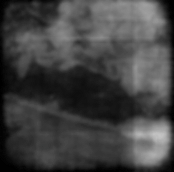
\includegraphics[scale=1.1]{./images/RESULTS/compare870/MSB.png}}&
\subfloat[MSBD]{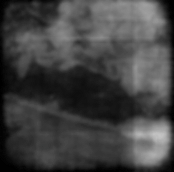
\includegraphics[scale=1.1]{./images/RESULTS/compare870/MSBD.png}}
\end{array}$
\end{center}

\caption{Proceso para MSBD en extracción 870-845.}
\label{pics:process}
\end{figure}
En las imágenes se muestran los resultados con base en los procedimientos explicados en el capítulo \ref{Capitulo2} y presentados en la Figura \ref{pics:squeme}.%Algoritmos
% Chapter Template
\chapter{Conclusiones} % Main chapter title
\label{Capitulo5} % Change X to a consecutive number; for referencing this chapter elsewhere, use \ref{ChapterX}
\lhead{\emph{Conclusiones}}

%----------------------------------------------------------------------------------------
%	SECTION 1
%----------------------------------------------------------------------------------------
Dentro de la descripción de la Hipotesis se menciona como objetivo lograr una mejora posterior al aplicar el procedimiento CTIS mediante filtrados diversos que puedieran eliminar ruido de las imágenes hiperespectrales resultantes. 

Mediante la utilización Mosaico Bayer y método de Malvar (vea \ref{capMalvar}) previo a la generación de imágenes de cubo hiperespectral, se pudo permitir que el resultado tuviera una mejora significante.
Después de obtener dicho resultado se aplica el método CTIS para obtener las imágenes y a estas imágenes se le aplica el desenfoque (vea capítulo \ref{CapBlur}) y la nitidez (véa \ref{capSharpender}) como último paso en el proceso.

Posterior a ello se aplicaron las series de Daubichies (vea la sección \ref{rDau}) que fueron descartados ya que no se presento algúna mejora notable al ser aplicado dejando el desenfoque y la nitidez como pasos definitivos.

La forma en que se comprobo la mejora fue visual, ya que por ser se tenían imagenes sin ruido con las cuales validar. Esto debido a que se trabajó directamente con imagenes abstraidas de la camara \ref{} con estructura CTIS.

Gracias a la aportación dada el presente proyecto se podrá dar una mejora con la cual será posible obtener un acercamiento a un producto con mayor madurez capaz de dar como resultado imagenes con mayor calidad(conservando detalles y eliminando ruido).


\begin{figure}[h]
\begin{center}$
\begin{array}{lll}
\subfloat[Original]{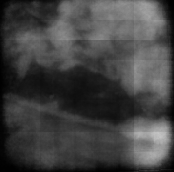
\includegraphics[scale=1.5]{./images/RESULTS/compare870/original.png}}&
\subfloat[MSB]{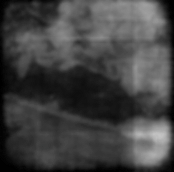
\includegraphics[scale=1.125]{./images/RESULTS/compare870/MSB.png}}
\end{array}$
\end{center}

\caption{Proceso para MSBD en extracción 870-845.}
\label{pics:process}
\end{figure}%Resultados

%----------------------------------------------------------------------------------------
%   GLOSSARY
%----------------------------------------------------------------------------------------
%\textit

glosario

RGB
snapshot
que consiste en un único tiempo de integración gracias a un conjunto de detectores. 
lente de colimación
RGGB
imagen Bayer
arreglo Bayer RGGB
interpolación cromática
interpolación bilineal
slit
patrón Bayer RGGB
Laplaciano


10 Denoising *
12 Nasa Airbone Visible *
17 Hyperspectral subspace identification *
18 model coordinates *
19 Medical Imaging *
22 Hyperspectral Subspace Identification * 
23 A Compressive Sensing and Unmixing Scheme for Hyperspectral Data Processing (extra2) *
27 Method of selecting the best classification bands from hyperspectral images based on genetic algorithm and rough set (extra6) *
28 Visual method for spectral band selection (extra7) *
31 Noise reduction of hyperspectral imagery using hybrid spatial-spectral derivative-domain wavelet shrinkage (extra10) *
32 Wavelet-based hyperspectral and multispectral image fusion (extra11) *%Glosario
\chapter{Glosario} % Main appendix title
\lhead{\emph{Glosario}}

\textbf{Interpolación Bilineal} 

La interpolación consiste en hallar un dato dentro de un intervalo en el que conocemos los valores en los extremos. La interpolación se dirá lineal cuando sólo se tomen dos puntos y cuadrática cuando se tomen tres.

\textbf{Interpolación Cromática} 

Un algoritmo de interpolación cromática (conocida en inglés como demosaicing o demosaicking) es un proceso digital de imagen utilizado para reconstruir una imagen en color mediante las muestras cromáticas incompletas adquiridas desde un sensor de imagen recubierto con un mosaico de filtro de color.

\textbf{Mosaico de Bayer} 

El filtro, máscara o mosaico de Bayer es un tipo de matriz de filtros, rojos verdes y azules, que se sitúa sobre un sensor digital de imagen para hacer llegar a cada fotodiodo la información de luminosidad correspondiente a una sección de los distintos colores primarios. 

\textbf{Laplaciano} 

 Es un operador diferencial elíptico de segundo orden, denotado como Δ, relacionado con ciertos problemas de minimización de ciertas magnitudes sobre un cierto dominio.

\textbf{Colimación} 

Es un sistema que a partir de un haz (de luz, de electrones, etc.) divergente obtiene un "haz" paralelo. Sirve para homogeneizar las trayectorias o rayos que, emitidos por una fuente, salen en todas direcciones y obtiene un chorro de partículas o conjunto de rayos con las mismas propiedades.

\textbf{patrón Bayer RGGB} 



\textbf{RGB} 

\textbf{RGGB} 

\textbf{slit} 

\textbf{snapshot} 

que consiste en un único tiempo de integración gracias a un conjunto de detectores. 

Aqui va la parte de anexos significativos para el proyecto. wdf aswdf sadf sadf safAqui va la parte de anexos significativos para el proyecto. wdf aswdf sadf sadf safAqui va la parte de anexos significativos para el proyecto. wdf aswdf sadf sadf safAqui va la parte de anexos significativos para el proyecto. wdf aswdf sadf sadf safAqui va la parte de anexos significativos para el proyecto. wdf aswdf sadf sadf safAqui va la parte de anexos significativos para el proyecto. wdf aswdf sadf sadf safAqui va la parte de anexos significativos para el proyecto. wdf aswdf sadf sadf safAqui va la parte de anexos significativos para el proyecto. wdf aswdf sadf sadf safAqui va la parte de anexos significativos para el proyecto. wdf aswdf sadf sadf safAqui va la parte de anexos significativos para el proyecto. wdf aswdf sadf sadf safAqui va la parte de anexos significativos para el proyecto. wdf aswdf sadf sadf safAqui va la parte de anexos significativos para el proyecto. wdf aswdf sadf sadf safAqui va la parte de anexos significativos para el proyecto. wdf aswdf sadf sadf safAqui va la parte de anexos significativos para el proyecto. wdf aswdf sadf sadf safAqui va la parte de anexos significativos para el proyecto. wdf aswdf sadf sadf safAqui va la parte de anexos significativos para el proyecto. wdf aswdf sadf sadf 

%----------------------------------------------------------------------------------------
%	THESIS CONTENT - APPENDICES
%----------------------------------------------------------------------------------------

\addtocontents{toc}{\vspace{2em}} % Add a gap in the Contents, for aesthetics

\appendix % Cue to tell LaTeX that the following 'chapters' are Appendices

% Include the appendices of the thesis as separate files from the Appendices folder
% Uncomment the lines as you write the Appendices

%\chapter{Glosario} % Main appendix title
\lhead{\emph{Glosario}}

\textbf{Interpolación Bilineal} 

La interpolación consiste en hallar un dato dentro de un intervalo en el que conocemos los valores en los extremos. La interpolación se dirá lineal cuando sólo se tomen dos puntos y cuadrática cuando se tomen tres.

\textbf{Interpolación Cromática} 

Un algoritmo de interpolación cromática (conocida en inglés como demosaicing o demosaicking) es un proceso digital de imagen utilizado para reconstruir una imagen en color mediante las muestras cromáticas incompletas adquiridas desde un sensor de imagen recubierto con un mosaico de filtro de color.

\textbf{Mosaico de Bayer} 

El filtro, máscara o mosaico de Bayer es un tipo de matriz de filtros, rojos verdes y azules, que se sitúa sobre un sensor digital de imagen para hacer llegar a cada fotodiodo la información de luminosidad correspondiente a una sección de los distintos colores primarios. 

\textbf{Laplaciano} 

 Es un operador diferencial elíptico de segundo orden, denotado como Δ, relacionado con ciertos problemas de minimización de ciertas magnitudes sobre un cierto dominio.

\textbf{Colimación} 

Es un sistema que a partir de un haz (de luz, de electrones, etc.) divergente obtiene un "haz" paralelo. Sirve para homogeneizar las trayectorias o rayos que, emitidos por una fuente, salen en todas direcciones y obtiene un chorro de partículas o conjunto de rayos con las mismas propiedades.

\textbf{patrón Bayer RGGB} 



\textbf{RGB} 

\textbf{RGGB} 

\textbf{slit} 

\textbf{snapshot} 

que consiste en un único tiempo de integración gracias a un conjunto de detectores. 

Aqui va la parte de anexos significativos para el proyecto. wdf aswdf sadf sadf safAqui va la parte de anexos significativos para el proyecto. wdf aswdf sadf sadf safAqui va la parte de anexos significativos para el proyecto. wdf aswdf sadf sadf safAqui va la parte de anexos significativos para el proyecto. wdf aswdf sadf sadf safAqui va la parte de anexos significativos para el proyecto. wdf aswdf sadf sadf safAqui va la parte de anexos significativos para el proyecto. wdf aswdf sadf sadf safAqui va la parte de anexos significativos para el proyecto. wdf aswdf sadf sadf safAqui va la parte de anexos significativos para el proyecto. wdf aswdf sadf sadf safAqui va la parte de anexos significativos para el proyecto. wdf aswdf sadf sadf safAqui va la parte de anexos significativos para el proyecto. wdf aswdf sadf sadf safAqui va la parte de anexos significativos para el proyecto. wdf aswdf sadf sadf safAqui va la parte de anexos significativos para el proyecto. wdf aswdf sadf sadf safAqui va la parte de anexos significativos para el proyecto. wdf aswdf sadf sadf safAqui va la parte de anexos significativos para el proyecto. wdf aswdf sadf sadf safAqui va la parte de anexos significativos para el proyecto. wdf aswdf sadf sadf safAqui va la parte de anexos significativos para el proyecto. wdf aswdf sadf sadf 
%\input{Appendices/AppendixB}
%\input{Appendices/AppendixC}

\addtocontents{toc}{\vspace{2em}} % Add a gap in the Contents, for aesthetics

\backmatter

%----------------------------------------------------------------------------------------
%	BIBLIOGRAPHY
%----------------------------------------------------------------------------------------

\lhead{\emph{Bibliografía}} % Change the page header to say "Bibliography"

\label{Bibliografia}

\input{references.bib}%References

\end{document}  

